\chapter{Matematyka dyskretna} 
\begin{definition}[Definicja permutacyjna wyznacznika]
Jeśli \(\field\) jest ciałem i \(n \in \natural\), to \textbf{wyznacznikiem} nazwiemy funkcję \(f : \fieldset^{n \times n}\) taką, że:

\[
f(A) = \sum_{\sigma \in S_n} \sgn(\sigma) \cdot A_{1, \; \sigma(1)} \cdot A_{2, \; \sigma(2)} \cdot A_{3, \; \sigma(3)} \cdot \dots \cdot A_{n, \; \sigma(n)} 
\]

gdzie \(A_{ij}\) oznacza komórkę macierzy znajdującą się w \(i\)-tym wierszu i \(j\)-tej kolumnie, a \(S_n\) oznacza zbiór wszystkich permutacji zbioru \(n\)-elementowego.

\end{definition}

\begin{definition}[Definicja ,,objętościowa'' wyznacznika]
Niech \(\field\) będzie ciałem i \(n \in \natural\). Ponadto, niech \(v_1, v_2, v_3, \dots, v_n \in \fieldset^{n}\). Wówczas tuplę \((v_1, v_2, v_3, \dots, v_n) \in (\fieldset^{n})^{n}\) możemy trywialnie utożsamić z macierzą \(M \in \fieldset^{n \times n}\) (i vice versa), poprzez utożsamienie każdego wektora \(\fieldset^{n}\) z pojedynczym wierszem tej macierzy.

Stosując taką notację, mówimy że funkcja \(f: \fieldset^{n \times n} \rightarrow \fieldset\) jest \textbf{wyznacznikiem}, jeśli spełnia następujące warunki: 

\begin{enumerate}
    \item \(f(v_1, v_2, \dots, \lambda v_i, \dots, v_n) = \lambda \cdot f(v_1, v_2, \dots, v_i, \dots, v_n) \)
    \item \(f(v_1, v_2, \dots, v_i + v_{i}', \dots, v_n) = f(v_1, v_2, \dots, v_i, \dots, v_n) + f(v_1, v_2, \dots, v_{i}', \dots, v_n) \)
    \item Jeżeli istnieje takie \(i\), że \(v_i = v_{i+1}\), to \(f(v_1, v_2, \dots, v_i, v_{i+1}, \dots v_n) = 0\)
    \item \(f\) na macierzy identycznościowej przyjmuje wartość \(1\). 
\end{enumerate}

Postulaty te wynikają z chęci stworzenia funkcji obliczającej zorientowaną objętość wielowymiarowego równoległościanu (opisywanego wektorami).

Można wykazać, że dla określonego \(n \in \natural\) istnieje dokładnie 1 funkcja spełniająca wyżej wymienione warunki. Definicja ta okazuje się być równoważna z tą wcześniejszą.

\end{definition}

Wyznacznik oznaczamy jako \(\det\).

\section{Zasada włączeń i wyłączeń. Przykłady zastosowań}
\begin{definition}[Definicja permutacyjna wyznacznika]
Jeśli \(\field\) jest ciałem i \(n \in \natural\), to \textbf{wyznacznikiem} nazwiemy funkcję \(f : \fieldset^{n \times n}\) taką, że:

\[
f(A) = \sum_{\sigma \in S_n} \sgn(\sigma) \cdot A_{1, \; \sigma(1)} \cdot A_{2, \; \sigma(2)} \cdot A_{3, \; \sigma(3)} \cdot \dots \cdot A_{n, \; \sigma(n)} 
\]

gdzie \(A_{ij}\) oznacza komórkę macierzy znajdującą się w \(i\)-tym wierszu i \(j\)-tej kolumnie, a \(S_n\) oznacza zbiór wszystkich permutacji zbioru \(n\)-elementowego.

\end{definition}

\begin{definition}[Definicja ,,objętościowa'' wyznacznika]
Niech \(\field\) będzie ciałem i \(n \in \natural\). Ponadto, niech \(v_1, v_2, v_3, \dots, v_n \in \fieldset^{n}\). Wówczas tuplę \((v_1, v_2, v_3, \dots, v_n) \in (\fieldset^{n})^{n}\) możemy trywialnie utożsamić z macierzą \(M \in \fieldset^{n \times n}\) (i vice versa), poprzez utożsamienie każdego wektora \(\fieldset^{n}\) z pojedynczym wierszem tej macierzy.

Stosując taką notację, mówimy że funkcja \(f: \fieldset^{n \times n} \rightarrow \fieldset\) jest \textbf{wyznacznikiem}, jeśli spełnia następujące warunki: 

\begin{enumerate}
    \item \(f(v_1, v_2, \dots, \lambda v_i, \dots, v_n) = \lambda \cdot f(v_1, v_2, \dots, v_i, \dots, v_n) \)
    \item \(f(v_1, v_2, \dots, v_i + v_{i}', \dots, v_n) = f(v_1, v_2, \dots, v_i, \dots, v_n) + f(v_1, v_2, \dots, v_{i}', \dots, v_n) \)
    \item Jeżeli istnieje takie \(i\), że \(v_i = v_{i+1}\), to \(f(v_1, v_2, \dots, v_i, v_{i+1}, \dots v_n) = 0\)
    \item \(f\) na macierzy identycznościowej przyjmuje wartość \(1\). 
\end{enumerate}

Postulaty te wynikają z chęci stworzenia funkcji obliczającej zorientowaną objętość wielowymiarowego równoległościanu (opisywanego wektorami).

Można wykazać, że dla określonego \(n \in \natural\) istnieje dokładnie 1 funkcja spełniająca wyżej wymienione warunki. Definicja ta okazuje się być równoważna z tą wcześniejszą.

\end{definition}

Wyznacznik oznaczamy jako \(\det\).
\begin{theorem}
Dla dowolnych zbiorów \(A, B, C\) zachodzi
\begin{equation*}
    \pars{A^B}^C \eqnum A^{B \times C}
\end{equation*}
\end{theorem}
\begin{proof}
Z~definicji --- konstruujemy bijekcję
\begin{equation*}
    \alpha\colon \pars{A^B}^C \function A^{B \times C}
\end{equation*}
Funkcja \(\alpha\)~przyjmuje funkcję \(C \function A^B\) i~zwraca funkcję \(B \times C \function A\). Zdefiniujmy \(\alpha\)~następująco:
\begin{equation*}
    \begin{split}
        \alpha\pars{f}
            &\coloneqq \pars{\text{taka funkcja \(\gamma\), że \(\gamma\pars{b, c} = \pars{f\pars{c}}\pars{b}\)}}\\
            &\coloneqq \set{\pars{\pars{b, c}, \pars{f\pars{c}}\pars{b}} : \pars{b, c} \in B \times C}
    \end{split}
\end{equation*}
Nadużywając trochę notacji, możemy to bardziej intuicyjnie zapisać jako
\begin{equation*}
    \pars{\alpha\pars{f}}\pars{b, c} \coloneqq \pars{f\pars{c}}\pars{b}
\end{equation*}
Musimy pokazać, że \(\alpha\)~bijekcją.
\begin{description}
    \item[Injektywność.] Weźmy różne \(f_1, f_2 \in \pars{A^B}^C\) i~pokażmy, że \(\alpha\pars{f_1} \neq \alpha\pars{f_2}\).

        Co to znaczy, że \(f_1, f_2\) są różne? To są funkcje \(C \function A^B\), więc gdy są różne, to na jakimś argumencie \(c_0 \in C\) przyjmują różne wartości:
        \begin{equation*}
            f_1\pars{c_0} \neq f_2\pars{c_0}
        \end{equation*}
        Ale to też są funkcje, tym razem \(B \function A\). Czyli skoro są różne, to na pewnym argumencie \(b_0 \in B\) przyjmują różne wartości:
        \begin{equation*}
            \pars{f_1\pars{c_0}}\pars{b_0} \neq \pars{f_2\pars{c_0}}\pars{b_0}
        \end{equation*}
        Możemy to zapisać za pomocą \(\alpha\)~jako
        \begin{equation*}
            \pars{\alpha\pars{f_1}}\pars{b_0, c_0} \neq \pars{\alpha\pars{f_2}}\pars{b_0, c_0}
        \end{equation*}
        Oznacza to, że funkcje \(\alpha\pars{f_1}, \alpha\pars{f_2}\colon B \times C \function \alpha\) przyjmują różne wartości na argumencie \(\pars{b_0, c_0} \in B \times C\). A~zatem są to różne funkcje \(\alpha\pars{f_1} \neq \alpha\pars{f_2}\), co właśnie chcieliśmy udowodnić.
    \item[Surjektywność.] Weźmy \(g \in A^{B \times C}\). Musimy pokazać, że istnieje \(f \in \pars{A^B}^C\) takie, że
        \begin{equation*}
            \alpha\pars{f} = g
        \end{equation*}
        Niewątpliwie, w~dziedzinie funkcji \(\alpha\)~znajduje się w~szczególności \(f_0\colon C \function A^B\)~zdefiniowane następująco
        \begin{equation*}
            \begin{split}
                f_0\pars{c}
                    &\coloneqq \pars{\text{taka funkcja \(\gamma\), że \(\gamma\pars{b} = g\pars{b, c}\)}}\\
                    &\coloneqq \set{\pars{b, g\pars{b, c}} : b \in B}
            \end{split}
        \end{equation*}
        co można, ponownie z~drobnym nadużyciem notacji można zapisać jako
        \begin{equation*}
            \pars{f_0\pars{c}}\pars{b} \coloneqq g\pars{b, c}
        \end{equation*}
        Zobaczmy, że dla dowolnej pary \(\pars{b_0, c_0} \in B \times C\) zachodzi
        \begin{align*}
            \pars{\alpha\pars{f_0}}\pars{b_0, c_0}
                &= \pars{f_0\pars{c_0}}\pars{b_0} && \text{z~definicji \(\alpha\)}\\
                &= g\pars{b_0, c_0} && \text{z~definicji \(f_0\)}
        \end{align*}
        Zatem istotnie \(\alpha\pars{f_0} = g\) jako funkcje.
\end{description}
\end{proof}
\begin{theorem}
Dla dowolnych zbiorów \(A, B, C\) zachodzi
\begin{equation*}
    \pars{A \times B}^C \eqnum A^C \times B^C
\end{equation*}
\end{theorem}
\begin{proof}
Korzystamy z~przemienności i~konstruujemy bijekcję
\begin{equation*}
    \alpha\colon A^C \times B^C \function \pars{A \times B}^C
\end{equation*}
Funkcja \(\alpha\)~przyjmuje parę funkcji \(\pars{C \function A, C \function B}\) i~zwraca funkcję \(C \function A \times B\). Definiujemy ją następująco:
\begin{equation*}
    \begin{split}
        \alpha\pars{f, g}
            &\coloneqq \pars{\text{taka funkcja \(\eta\), że \(\eta\pars{c} = \pars{f\pars{c}, g\pars{c}}\)}}\\
            &\coloneqq \set{\pars{c, \pars{f\pars{c}, g\pars{c}}} : c \in C}
    \end{split}
\end{equation*}
Inaczej:
\begin{equation*}
    \pars{\alpha\pars{f, g}}\pars{c} = \pars{f\pars{c}, g\pars{c}}
\end{equation*}
Musimy pokazać, że \(\alpha\)~jest bijekcją.
\begin{description}
    \item[Injektywność.] Weźmy różne pary \(\pars{f_1, g_1}, \pars{f_2, g_2} \in A^C \times B^C\). Skoro są to różne pary funkcji, to istnieje takie \(c_0 \in C\), że \(f_1\pars{c_0} \neq f_2\pars{c_0}\) lub istnieje takie \(c_0' \in C\), że \(g_1\pars{c_0'} \neq g_2\pars{c_0'}\). Bez straty ogólności, przyjmijmy pierwszą opcję. Widzimy, że
    \begin{equation*}
        \pars{\alpha\pars{f_1, g_1}}\pars{c_0} = \pars{f_1\pars{c_0}, g_1\pars{c_0}} \neq \pars{f_2\pars{c_0}, g_2\pars{c_0}} = \pars{\alpha\pars{f_2, g_2}}\pars{c_0}
    \end{equation*}
    Oznacza to, że \(\alpha\pars{f_1, g_1}\) i~\(\alpha\pars{f_2, g_2}\) są różnymi funkcjami --- tak, jak chcieliśmy.
    \item[Surjektywność.] Weźmy \(h \in \pars{A \times B}^C\). Musimy pokazać, że istnieje para \(\pars{f_0, g_0} \in A^C \times B^C\) taka, że
        \begin{equation*}
            \alpha\pars{f_0, g_0} = h
        \end{equation*}
        Weźmy
        \begin{gather*}
            f_0\colon C \function A\\
            f_0\pars{c} \coloneqq \text{lewy element pary \(h\pars{c}\)}
        \end{gather*}
        oraz
        \begin{gather*}
            g_0\colon C \function B\\
            g_0\pars{c} \coloneqq \text{prawy element pary \(h\pars{c}\)}
        \end{gather*}
        Teraz dla dowolnego \(c_0 \in C\) mamy
        \begin{equation*}
            \pars{\alpha\pars{f_0, g_0}}\pars{c_0}
                = \pars{f_0\pars{c_0}, g_0\pars{c_0}}
                = \pars{\text{lewy z~\(h\pars{c_0}\)}, \text{prawy z~\(h\pars{c_0}\)}}
                = h\pars{c_0}
        \end{equation*}
        co dowodzi, że \(\alpha\pars{f_0, g_0} = h\) jako funkcje.
        
        Jako bonus możemy zastanowić się, jak teoriomnogościowo wyciągać lewy i~prawy element pary uporządkowanej. Wykorzystamy definicję \ref{mfi:cartesian_and_relations:cartesian_definitions:def:ordered_pair}.
        \begin{itemize}
            \item \(\bigcup\bigcap p\) jest lewym elementem pary \(p\)
                \begin{equation*}
                    p = \pars{a, b} = \set{\set{a}, \set{a, b}} \overset{\bigcap}{\longrightarrow} \set{a} \overset{\bigcup}{\longrightarrow} a
                \end{equation*}
            \item \(\bigcup\pars{\bigcup p \setminus \bigcap p}\) jest prawym elementem pary \(p\)
                \begin{equation*}
                    p = \pars{a, b} = \set{\set{a}, \set{a, b}} \overset{\bigcap}{\longrightarrow} \set{a} \overset{\bigcup \setminus \pars{\mathord{\cdot}}}{\longrightarrow} \set{a, b} \setminus \set{a} = \set{b} \overset{\bigcup}{\longrightarrow} b
                \end{equation*}
        \end{itemize}
\end{description}
\end{proof}



\section{Porządki częściowe, Twierdzenia Dilwortha i Spernera}
\begin{definition}[Definicja permutacyjna wyznacznika]
Jeśli \(\field\) jest ciałem i \(n \in \natural\), to \textbf{wyznacznikiem} nazwiemy funkcję \(f : \fieldset^{n \times n}\) taką, że:

\[
f(A) = \sum_{\sigma \in S_n} \sgn(\sigma) \cdot A_{1, \; \sigma(1)} \cdot A_{2, \; \sigma(2)} \cdot A_{3, \; \sigma(3)} \cdot \dots \cdot A_{n, \; \sigma(n)} 
\]

gdzie \(A_{ij}\) oznacza komórkę macierzy znajdującą się w \(i\)-tym wierszu i \(j\)-tej kolumnie, a \(S_n\) oznacza zbiór wszystkich permutacji zbioru \(n\)-elementowego.

\end{definition}

\begin{definition}[Definicja ,,objętościowa'' wyznacznika]
Niech \(\field\) będzie ciałem i \(n \in \natural\). Ponadto, niech \(v_1, v_2, v_3, \dots, v_n \in \fieldset^{n}\). Wówczas tuplę \((v_1, v_2, v_3, \dots, v_n) \in (\fieldset^{n})^{n}\) możemy trywialnie utożsamić z macierzą \(M \in \fieldset^{n \times n}\) (i vice versa), poprzez utożsamienie każdego wektora \(\fieldset^{n}\) z pojedynczym wierszem tej macierzy.

Stosując taką notację, mówimy że funkcja \(f: \fieldset^{n \times n} \rightarrow \fieldset\) jest \textbf{wyznacznikiem}, jeśli spełnia następujące warunki: 

\begin{enumerate}
    \item \(f(v_1, v_2, \dots, \lambda v_i, \dots, v_n) = \lambda \cdot f(v_1, v_2, \dots, v_i, \dots, v_n) \)
    \item \(f(v_1, v_2, \dots, v_i + v_{i}', \dots, v_n) = f(v_1, v_2, \dots, v_i, \dots, v_n) + f(v_1, v_2, \dots, v_{i}', \dots, v_n) \)
    \item Jeżeli istnieje takie \(i\), że \(v_i = v_{i+1}\), to \(f(v_1, v_2, \dots, v_i, v_{i+1}, \dots v_n) = 0\)
    \item \(f\) na macierzy identycznościowej przyjmuje wartość \(1\). 
\end{enumerate}

Postulaty te wynikają z chęci stworzenia funkcji obliczającej zorientowaną objętość wielowymiarowego równoległościanu (opisywanego wektorami).

Można wykazać, że dla określonego \(n \in \natural\) istnieje dokładnie 1 funkcja spełniająca wyżej wymienione warunki. Definicja ta okazuje się być równoważna z tą wcześniejszą.

\end{definition}

Wyznacznik oznaczamy jako \(\det\).
\begin{theorem}
Dla dowolnych zbiorów \(A, B, C\) zachodzi
\begin{equation*}
    \pars{A^B}^C \eqnum A^{B \times C}
\end{equation*}
\end{theorem}
\begin{proof}
Z~definicji --- konstruujemy bijekcję
\begin{equation*}
    \alpha\colon \pars{A^B}^C \function A^{B \times C}
\end{equation*}
Funkcja \(\alpha\)~przyjmuje funkcję \(C \function A^B\) i~zwraca funkcję \(B \times C \function A\). Zdefiniujmy \(\alpha\)~następująco:
\begin{equation*}
    \begin{split}
        \alpha\pars{f}
            &\coloneqq \pars{\text{taka funkcja \(\gamma\), że \(\gamma\pars{b, c} = \pars{f\pars{c}}\pars{b}\)}}\\
            &\coloneqq \set{\pars{\pars{b, c}, \pars{f\pars{c}}\pars{b}} : \pars{b, c} \in B \times C}
    \end{split}
\end{equation*}
Nadużywając trochę notacji, możemy to bardziej intuicyjnie zapisać jako
\begin{equation*}
    \pars{\alpha\pars{f}}\pars{b, c} \coloneqq \pars{f\pars{c}}\pars{b}
\end{equation*}
Musimy pokazać, że \(\alpha\)~bijekcją.
\begin{description}
    \item[Injektywność.] Weźmy różne \(f_1, f_2 \in \pars{A^B}^C\) i~pokażmy, że \(\alpha\pars{f_1} \neq \alpha\pars{f_2}\).

        Co to znaczy, że \(f_1, f_2\) są różne? To są funkcje \(C \function A^B\), więc gdy są różne, to na jakimś argumencie \(c_0 \in C\) przyjmują różne wartości:
        \begin{equation*}
            f_1\pars{c_0} \neq f_2\pars{c_0}
        \end{equation*}
        Ale to też są funkcje, tym razem \(B \function A\). Czyli skoro są różne, to na pewnym argumencie \(b_0 \in B\) przyjmują różne wartości:
        \begin{equation*}
            \pars{f_1\pars{c_0}}\pars{b_0} \neq \pars{f_2\pars{c_0}}\pars{b_0}
        \end{equation*}
        Możemy to zapisać za pomocą \(\alpha\)~jako
        \begin{equation*}
            \pars{\alpha\pars{f_1}}\pars{b_0, c_0} \neq \pars{\alpha\pars{f_2}}\pars{b_0, c_0}
        \end{equation*}
        Oznacza to, że funkcje \(\alpha\pars{f_1}, \alpha\pars{f_2}\colon B \times C \function \alpha\) przyjmują różne wartości na argumencie \(\pars{b_0, c_0} \in B \times C\). A~zatem są to różne funkcje \(\alpha\pars{f_1} \neq \alpha\pars{f_2}\), co właśnie chcieliśmy udowodnić.
    \item[Surjektywność.] Weźmy \(g \in A^{B \times C}\). Musimy pokazać, że istnieje \(f \in \pars{A^B}^C\) takie, że
        \begin{equation*}
            \alpha\pars{f} = g
        \end{equation*}
        Niewątpliwie, w~dziedzinie funkcji \(\alpha\)~znajduje się w~szczególności \(f_0\colon C \function A^B\)~zdefiniowane następująco
        \begin{equation*}
            \begin{split}
                f_0\pars{c}
                    &\coloneqq \pars{\text{taka funkcja \(\gamma\), że \(\gamma\pars{b} = g\pars{b, c}\)}}\\
                    &\coloneqq \set{\pars{b, g\pars{b, c}} : b \in B}
            \end{split}
        \end{equation*}
        co można, ponownie z~drobnym nadużyciem notacji można zapisać jako
        \begin{equation*}
            \pars{f_0\pars{c}}\pars{b} \coloneqq g\pars{b, c}
        \end{equation*}
        Zobaczmy, że dla dowolnej pary \(\pars{b_0, c_0} \in B \times C\) zachodzi
        \begin{align*}
            \pars{\alpha\pars{f_0}}\pars{b_0, c_0}
                &= \pars{f_0\pars{c_0}}\pars{b_0} && \text{z~definicji \(\alpha\)}\\
                &= g\pars{b_0, c_0} && \text{z~definicji \(f_0\)}
        \end{align*}
        Zatem istotnie \(\alpha\pars{f_0} = g\) jako funkcje.
\end{description}
\end{proof}
\begin{theorem}
Dla dowolnych zbiorów \(A, B, C\) zachodzi
\begin{equation*}
    \pars{A \times B}^C \eqnum A^C \times B^C
\end{equation*}
\end{theorem}
\begin{proof}
Korzystamy z~przemienności i~konstruujemy bijekcję
\begin{equation*}
    \alpha\colon A^C \times B^C \function \pars{A \times B}^C
\end{equation*}
Funkcja \(\alpha\)~przyjmuje parę funkcji \(\pars{C \function A, C \function B}\) i~zwraca funkcję \(C \function A \times B\). Definiujemy ją następująco:
\begin{equation*}
    \begin{split}
        \alpha\pars{f, g}
            &\coloneqq \pars{\text{taka funkcja \(\eta\), że \(\eta\pars{c} = \pars{f\pars{c}, g\pars{c}}\)}}\\
            &\coloneqq \set{\pars{c, \pars{f\pars{c}, g\pars{c}}} : c \in C}
    \end{split}
\end{equation*}
Inaczej:
\begin{equation*}
    \pars{\alpha\pars{f, g}}\pars{c} = \pars{f\pars{c}, g\pars{c}}
\end{equation*}
Musimy pokazać, że \(\alpha\)~jest bijekcją.
\begin{description}
    \item[Injektywność.] Weźmy różne pary \(\pars{f_1, g_1}, \pars{f_2, g_2} \in A^C \times B^C\). Skoro są to różne pary funkcji, to istnieje takie \(c_0 \in C\), że \(f_1\pars{c_0} \neq f_2\pars{c_0}\) lub istnieje takie \(c_0' \in C\), że \(g_1\pars{c_0'} \neq g_2\pars{c_0'}\). Bez straty ogólności, przyjmijmy pierwszą opcję. Widzimy, że
    \begin{equation*}
        \pars{\alpha\pars{f_1, g_1}}\pars{c_0} = \pars{f_1\pars{c_0}, g_1\pars{c_0}} \neq \pars{f_2\pars{c_0}, g_2\pars{c_0}} = \pars{\alpha\pars{f_2, g_2}}\pars{c_0}
    \end{equation*}
    Oznacza to, że \(\alpha\pars{f_1, g_1}\) i~\(\alpha\pars{f_2, g_2}\) są różnymi funkcjami --- tak, jak chcieliśmy.
    \item[Surjektywność.] Weźmy \(h \in \pars{A \times B}^C\). Musimy pokazać, że istnieje para \(\pars{f_0, g_0} \in A^C \times B^C\) taka, że
        \begin{equation*}
            \alpha\pars{f_0, g_0} = h
        \end{equation*}
        Weźmy
        \begin{gather*}
            f_0\colon C \function A\\
            f_0\pars{c} \coloneqq \text{lewy element pary \(h\pars{c}\)}
        \end{gather*}
        oraz
        \begin{gather*}
            g_0\colon C \function B\\
            g_0\pars{c} \coloneqq \text{prawy element pary \(h\pars{c}\)}
        \end{gather*}
        Teraz dla dowolnego \(c_0 \in C\) mamy
        \begin{equation*}
            \pars{\alpha\pars{f_0, g_0}}\pars{c_0}
                = \pars{f_0\pars{c_0}, g_0\pars{c_0}}
                = \pars{\text{lewy z~\(h\pars{c_0}\)}, \text{prawy z~\(h\pars{c_0}\)}}
                = h\pars{c_0}
        \end{equation*}
        co dowodzi, że \(\alpha\pars{f_0, g_0} = h\) jako funkcje.
        
        Jako bonus możemy zastanowić się, jak teoriomnogościowo wyciągać lewy i~prawy element pary uporządkowanej. Wykorzystamy definicję \ref{mfi:cartesian_and_relations:cartesian_definitions:def:ordered_pair}.
        \begin{itemize}
            \item \(\bigcup\bigcap p\) jest lewym elementem pary \(p\)
                \begin{equation*}
                    p = \pars{a, b} = \set{\set{a}, \set{a, b}} \overset{\bigcap}{\longrightarrow} \set{a} \overset{\bigcup}{\longrightarrow} a
                \end{equation*}
            \item \(\bigcup\pars{\bigcup p \setminus \bigcap p}\) jest prawym elementem pary \(p\)
                \begin{equation*}
                    p = \pars{a, b} = \set{\set{a}, \set{a, b}} \overset{\bigcap}{\longrightarrow} \set{a} \overset{\bigcup \setminus \pars{\mathord{\cdot}}}{\longrightarrow} \set{a, b} \setminus \set{a} = \set{b} \overset{\bigcup}{\longrightarrow} b
                \end{equation*}
        \end{itemize}
\end{description}
\end{proof}



\section{Twierdzenie Ramseya. Przykłady zastosowań}
\begin{definition}[Definicja permutacyjna wyznacznika]
Jeśli \(\field\) jest ciałem i \(n \in \natural\), to \textbf{wyznacznikiem} nazwiemy funkcję \(f : \fieldset^{n \times n}\) taką, że:

\[
f(A) = \sum_{\sigma \in S_n} \sgn(\sigma) \cdot A_{1, \; \sigma(1)} \cdot A_{2, \; \sigma(2)} \cdot A_{3, \; \sigma(3)} \cdot \dots \cdot A_{n, \; \sigma(n)} 
\]

gdzie \(A_{ij}\) oznacza komórkę macierzy znajdującą się w \(i\)-tym wierszu i \(j\)-tej kolumnie, a \(S_n\) oznacza zbiór wszystkich permutacji zbioru \(n\)-elementowego.

\end{definition}

\begin{definition}[Definicja ,,objętościowa'' wyznacznika]
Niech \(\field\) będzie ciałem i \(n \in \natural\). Ponadto, niech \(v_1, v_2, v_3, \dots, v_n \in \fieldset^{n}\). Wówczas tuplę \((v_1, v_2, v_3, \dots, v_n) \in (\fieldset^{n})^{n}\) możemy trywialnie utożsamić z macierzą \(M \in \fieldset^{n \times n}\) (i vice versa), poprzez utożsamienie każdego wektora \(\fieldset^{n}\) z pojedynczym wierszem tej macierzy.

Stosując taką notację, mówimy że funkcja \(f: \fieldset^{n \times n} \rightarrow \fieldset\) jest \textbf{wyznacznikiem}, jeśli spełnia następujące warunki: 

\begin{enumerate}
    \item \(f(v_1, v_2, \dots, \lambda v_i, \dots, v_n) = \lambda \cdot f(v_1, v_2, \dots, v_i, \dots, v_n) \)
    \item \(f(v_1, v_2, \dots, v_i + v_{i}', \dots, v_n) = f(v_1, v_2, \dots, v_i, \dots, v_n) + f(v_1, v_2, \dots, v_{i}', \dots, v_n) \)
    \item Jeżeli istnieje takie \(i\), że \(v_i = v_{i+1}\), to \(f(v_1, v_2, \dots, v_i, v_{i+1}, \dots v_n) = 0\)
    \item \(f\) na macierzy identycznościowej przyjmuje wartość \(1\). 
\end{enumerate}

Postulaty te wynikają z chęci stworzenia funkcji obliczającej zorientowaną objętość wielowymiarowego równoległościanu (opisywanego wektorami).

Można wykazać, że dla określonego \(n \in \natural\) istnieje dokładnie 1 funkcja spełniająca wyżej wymienione warunki. Definicja ta okazuje się być równoważna z tą wcześniejszą.

\end{definition}

Wyznacznik oznaczamy jako \(\det\).
\begin{theorem}
Dla dowolnych zbiorów \(A, B, C\) zachodzi
\begin{equation*}
    \pars{A^B}^C \eqnum A^{B \times C}
\end{equation*}
\end{theorem}
\begin{proof}
Z~definicji --- konstruujemy bijekcję
\begin{equation*}
    \alpha\colon \pars{A^B}^C \function A^{B \times C}
\end{equation*}
Funkcja \(\alpha\)~przyjmuje funkcję \(C \function A^B\) i~zwraca funkcję \(B \times C \function A\). Zdefiniujmy \(\alpha\)~następująco:
\begin{equation*}
    \begin{split}
        \alpha\pars{f}
            &\coloneqq \pars{\text{taka funkcja \(\gamma\), że \(\gamma\pars{b, c} = \pars{f\pars{c}}\pars{b}\)}}\\
            &\coloneqq \set{\pars{\pars{b, c}, \pars{f\pars{c}}\pars{b}} : \pars{b, c} \in B \times C}
    \end{split}
\end{equation*}
Nadużywając trochę notacji, możemy to bardziej intuicyjnie zapisać jako
\begin{equation*}
    \pars{\alpha\pars{f}}\pars{b, c} \coloneqq \pars{f\pars{c}}\pars{b}
\end{equation*}
Musimy pokazać, że \(\alpha\)~bijekcją.
\begin{description}
    \item[Injektywność.] Weźmy różne \(f_1, f_2 \in \pars{A^B}^C\) i~pokażmy, że \(\alpha\pars{f_1} \neq \alpha\pars{f_2}\).

        Co to znaczy, że \(f_1, f_2\) są różne? To są funkcje \(C \function A^B\), więc gdy są różne, to na jakimś argumencie \(c_0 \in C\) przyjmują różne wartości:
        \begin{equation*}
            f_1\pars{c_0} \neq f_2\pars{c_0}
        \end{equation*}
        Ale to też są funkcje, tym razem \(B \function A\). Czyli skoro są różne, to na pewnym argumencie \(b_0 \in B\) przyjmują różne wartości:
        \begin{equation*}
            \pars{f_1\pars{c_0}}\pars{b_0} \neq \pars{f_2\pars{c_0}}\pars{b_0}
        \end{equation*}
        Możemy to zapisać za pomocą \(\alpha\)~jako
        \begin{equation*}
            \pars{\alpha\pars{f_1}}\pars{b_0, c_0} \neq \pars{\alpha\pars{f_2}}\pars{b_0, c_0}
        \end{equation*}
        Oznacza to, że funkcje \(\alpha\pars{f_1}, \alpha\pars{f_2}\colon B \times C \function \alpha\) przyjmują różne wartości na argumencie \(\pars{b_0, c_0} \in B \times C\). A~zatem są to różne funkcje \(\alpha\pars{f_1} \neq \alpha\pars{f_2}\), co właśnie chcieliśmy udowodnić.
    \item[Surjektywność.] Weźmy \(g \in A^{B \times C}\). Musimy pokazać, że istnieje \(f \in \pars{A^B}^C\) takie, że
        \begin{equation*}
            \alpha\pars{f} = g
        \end{equation*}
        Niewątpliwie, w~dziedzinie funkcji \(\alpha\)~znajduje się w~szczególności \(f_0\colon C \function A^B\)~zdefiniowane następująco
        \begin{equation*}
            \begin{split}
                f_0\pars{c}
                    &\coloneqq \pars{\text{taka funkcja \(\gamma\), że \(\gamma\pars{b} = g\pars{b, c}\)}}\\
                    &\coloneqq \set{\pars{b, g\pars{b, c}} : b \in B}
            \end{split}
        \end{equation*}
        co można, ponownie z~drobnym nadużyciem notacji można zapisać jako
        \begin{equation*}
            \pars{f_0\pars{c}}\pars{b} \coloneqq g\pars{b, c}
        \end{equation*}
        Zobaczmy, że dla dowolnej pary \(\pars{b_0, c_0} \in B \times C\) zachodzi
        \begin{align*}
            \pars{\alpha\pars{f_0}}\pars{b_0, c_0}
                &= \pars{f_0\pars{c_0}}\pars{b_0} && \text{z~definicji \(\alpha\)}\\
                &= g\pars{b_0, c_0} && \text{z~definicji \(f_0\)}
        \end{align*}
        Zatem istotnie \(\alpha\pars{f_0} = g\) jako funkcje.
\end{description}
\end{proof}
\begin{theorem}
Dla dowolnych zbiorów \(A, B, C\) zachodzi
\begin{equation*}
    \pars{A \times B}^C \eqnum A^C \times B^C
\end{equation*}
\end{theorem}
\begin{proof}
Korzystamy z~przemienności i~konstruujemy bijekcję
\begin{equation*}
    \alpha\colon A^C \times B^C \function \pars{A \times B}^C
\end{equation*}
Funkcja \(\alpha\)~przyjmuje parę funkcji \(\pars{C \function A, C \function B}\) i~zwraca funkcję \(C \function A \times B\). Definiujemy ją następująco:
\begin{equation*}
    \begin{split}
        \alpha\pars{f, g}
            &\coloneqq \pars{\text{taka funkcja \(\eta\), że \(\eta\pars{c} = \pars{f\pars{c}, g\pars{c}}\)}}\\
            &\coloneqq \set{\pars{c, \pars{f\pars{c}, g\pars{c}}} : c \in C}
    \end{split}
\end{equation*}
Inaczej:
\begin{equation*}
    \pars{\alpha\pars{f, g}}\pars{c} = \pars{f\pars{c}, g\pars{c}}
\end{equation*}
Musimy pokazać, że \(\alpha\)~jest bijekcją.
\begin{description}
    \item[Injektywność.] Weźmy różne pary \(\pars{f_1, g_1}, \pars{f_2, g_2} \in A^C \times B^C\). Skoro są to różne pary funkcji, to istnieje takie \(c_0 \in C\), że \(f_1\pars{c_0} \neq f_2\pars{c_0}\) lub istnieje takie \(c_0' \in C\), że \(g_1\pars{c_0'} \neq g_2\pars{c_0'}\). Bez straty ogólności, przyjmijmy pierwszą opcję. Widzimy, że
    \begin{equation*}
        \pars{\alpha\pars{f_1, g_1}}\pars{c_0} = \pars{f_1\pars{c_0}, g_1\pars{c_0}} \neq \pars{f_2\pars{c_0}, g_2\pars{c_0}} = \pars{\alpha\pars{f_2, g_2}}\pars{c_0}
    \end{equation*}
    Oznacza to, że \(\alpha\pars{f_1, g_1}\) i~\(\alpha\pars{f_2, g_2}\) są różnymi funkcjami --- tak, jak chcieliśmy.
    \item[Surjektywność.] Weźmy \(h \in \pars{A \times B}^C\). Musimy pokazać, że istnieje para \(\pars{f_0, g_0} \in A^C \times B^C\) taka, że
        \begin{equation*}
            \alpha\pars{f_0, g_0} = h
        \end{equation*}
        Weźmy
        \begin{gather*}
            f_0\colon C \function A\\
            f_0\pars{c} \coloneqq \text{lewy element pary \(h\pars{c}\)}
        \end{gather*}
        oraz
        \begin{gather*}
            g_0\colon C \function B\\
            g_0\pars{c} \coloneqq \text{prawy element pary \(h\pars{c}\)}
        \end{gather*}
        Teraz dla dowolnego \(c_0 \in C\) mamy
        \begin{equation*}
            \pars{\alpha\pars{f_0, g_0}}\pars{c_0}
                = \pars{f_0\pars{c_0}, g_0\pars{c_0}}
                = \pars{\text{lewy z~\(h\pars{c_0}\)}, \text{prawy z~\(h\pars{c_0}\)}}
                = h\pars{c_0}
        \end{equation*}
        co dowodzi, że \(\alpha\pars{f_0, g_0} = h\) jako funkcje.
        
        Jako bonus możemy zastanowić się, jak teoriomnogościowo wyciągać lewy i~prawy element pary uporządkowanej. Wykorzystamy definicję \ref{mfi:cartesian_and_relations:cartesian_definitions:def:ordered_pair}.
        \begin{itemize}
            \item \(\bigcup\bigcap p\) jest lewym elementem pary \(p\)
                \begin{equation*}
                    p = \pars{a, b} = \set{\set{a}, \set{a, b}} \overset{\bigcap}{\longrightarrow} \set{a} \overset{\bigcup}{\longrightarrow} a
                \end{equation*}
            \item \(\bigcup\pars{\bigcup p \setminus \bigcap p}\) jest prawym elementem pary \(p\)
                \begin{equation*}
                    p = \pars{a, b} = \set{\set{a}, \set{a, b}} \overset{\bigcap}{\longrightarrow} \set{a} \overset{\bigcup \setminus \pars{\mathord{\cdot}}}{\longrightarrow} \set{a, b} \setminus \set{a} = \set{b} \overset{\bigcup}{\longrightarrow} b
                \end{equation*}
        \end{itemize}
\end{description}
\end{proof}



\section{Funkcje tworzące. Wyznaczanie liczb Fibonacciego za pomocą funkcji tworzących}
\begin{definition}[Definicja permutacyjna wyznacznika]
Jeśli \(\field\) jest ciałem i \(n \in \natural\), to \textbf{wyznacznikiem} nazwiemy funkcję \(f : \fieldset^{n \times n}\) taką, że:

\[
f(A) = \sum_{\sigma \in S_n} \sgn(\sigma) \cdot A_{1, \; \sigma(1)} \cdot A_{2, \; \sigma(2)} \cdot A_{3, \; \sigma(3)} \cdot \dots \cdot A_{n, \; \sigma(n)} 
\]

gdzie \(A_{ij}\) oznacza komórkę macierzy znajdującą się w \(i\)-tym wierszu i \(j\)-tej kolumnie, a \(S_n\) oznacza zbiór wszystkich permutacji zbioru \(n\)-elementowego.

\end{definition}

\begin{definition}[Definicja ,,objętościowa'' wyznacznika]
Niech \(\field\) będzie ciałem i \(n \in \natural\). Ponadto, niech \(v_1, v_2, v_3, \dots, v_n \in \fieldset^{n}\). Wówczas tuplę \((v_1, v_2, v_3, \dots, v_n) \in (\fieldset^{n})^{n}\) możemy trywialnie utożsamić z macierzą \(M \in \fieldset^{n \times n}\) (i vice versa), poprzez utożsamienie każdego wektora \(\fieldset^{n}\) z pojedynczym wierszem tej macierzy.

Stosując taką notację, mówimy że funkcja \(f: \fieldset^{n \times n} \rightarrow \fieldset\) jest \textbf{wyznacznikiem}, jeśli spełnia następujące warunki: 

\begin{enumerate}
    \item \(f(v_1, v_2, \dots, \lambda v_i, \dots, v_n) = \lambda \cdot f(v_1, v_2, \dots, v_i, \dots, v_n) \)
    \item \(f(v_1, v_2, \dots, v_i + v_{i}', \dots, v_n) = f(v_1, v_2, \dots, v_i, \dots, v_n) + f(v_1, v_2, \dots, v_{i}', \dots, v_n) \)
    \item Jeżeli istnieje takie \(i\), że \(v_i = v_{i+1}\), to \(f(v_1, v_2, \dots, v_i, v_{i+1}, \dots v_n) = 0\)
    \item \(f\) na macierzy identycznościowej przyjmuje wartość \(1\). 
\end{enumerate}

Postulaty te wynikają z chęci stworzenia funkcji obliczającej zorientowaną objętość wielowymiarowego równoległościanu (opisywanego wektorami).

Można wykazać, że dla określonego \(n \in \natural\) istnieje dokładnie 1 funkcja spełniająca wyżej wymienione warunki. Definicja ta okazuje się być równoważna z tą wcześniejszą.

\end{definition}

Wyznacznik oznaczamy jako \(\det\).
\begin{theorem}
Dla dowolnych zbiorów \(A, B, C\) zachodzi
\begin{equation*}
    \pars{A^B}^C \eqnum A^{B \times C}
\end{equation*}
\end{theorem}
\begin{proof}
Z~definicji --- konstruujemy bijekcję
\begin{equation*}
    \alpha\colon \pars{A^B}^C \function A^{B \times C}
\end{equation*}
Funkcja \(\alpha\)~przyjmuje funkcję \(C \function A^B\) i~zwraca funkcję \(B \times C \function A\). Zdefiniujmy \(\alpha\)~następująco:
\begin{equation*}
    \begin{split}
        \alpha\pars{f}
            &\coloneqq \pars{\text{taka funkcja \(\gamma\), że \(\gamma\pars{b, c} = \pars{f\pars{c}}\pars{b}\)}}\\
            &\coloneqq \set{\pars{\pars{b, c}, \pars{f\pars{c}}\pars{b}} : \pars{b, c} \in B \times C}
    \end{split}
\end{equation*}
Nadużywając trochę notacji, możemy to bardziej intuicyjnie zapisać jako
\begin{equation*}
    \pars{\alpha\pars{f}}\pars{b, c} \coloneqq \pars{f\pars{c}}\pars{b}
\end{equation*}
Musimy pokazać, że \(\alpha\)~bijekcją.
\begin{description}
    \item[Injektywność.] Weźmy różne \(f_1, f_2 \in \pars{A^B}^C\) i~pokażmy, że \(\alpha\pars{f_1} \neq \alpha\pars{f_2}\).

        Co to znaczy, że \(f_1, f_2\) są różne? To są funkcje \(C \function A^B\), więc gdy są różne, to na jakimś argumencie \(c_0 \in C\) przyjmują różne wartości:
        \begin{equation*}
            f_1\pars{c_0} \neq f_2\pars{c_0}
        \end{equation*}
        Ale to też są funkcje, tym razem \(B \function A\). Czyli skoro są różne, to na pewnym argumencie \(b_0 \in B\) przyjmują różne wartości:
        \begin{equation*}
            \pars{f_1\pars{c_0}}\pars{b_0} \neq \pars{f_2\pars{c_0}}\pars{b_0}
        \end{equation*}
        Możemy to zapisać za pomocą \(\alpha\)~jako
        \begin{equation*}
            \pars{\alpha\pars{f_1}}\pars{b_0, c_0} \neq \pars{\alpha\pars{f_2}}\pars{b_0, c_0}
        \end{equation*}
        Oznacza to, że funkcje \(\alpha\pars{f_1}, \alpha\pars{f_2}\colon B \times C \function \alpha\) przyjmują różne wartości na argumencie \(\pars{b_0, c_0} \in B \times C\). A~zatem są to różne funkcje \(\alpha\pars{f_1} \neq \alpha\pars{f_2}\), co właśnie chcieliśmy udowodnić.
    \item[Surjektywność.] Weźmy \(g \in A^{B \times C}\). Musimy pokazać, że istnieje \(f \in \pars{A^B}^C\) takie, że
        \begin{equation*}
            \alpha\pars{f} = g
        \end{equation*}
        Niewątpliwie, w~dziedzinie funkcji \(\alpha\)~znajduje się w~szczególności \(f_0\colon C \function A^B\)~zdefiniowane następująco
        \begin{equation*}
            \begin{split}
                f_0\pars{c}
                    &\coloneqq \pars{\text{taka funkcja \(\gamma\), że \(\gamma\pars{b} = g\pars{b, c}\)}}\\
                    &\coloneqq \set{\pars{b, g\pars{b, c}} : b \in B}
            \end{split}
        \end{equation*}
        co można, ponownie z~drobnym nadużyciem notacji można zapisać jako
        \begin{equation*}
            \pars{f_0\pars{c}}\pars{b} \coloneqq g\pars{b, c}
        \end{equation*}
        Zobaczmy, że dla dowolnej pary \(\pars{b_0, c_0} \in B \times C\) zachodzi
        \begin{align*}
            \pars{\alpha\pars{f_0}}\pars{b_0, c_0}
                &= \pars{f_0\pars{c_0}}\pars{b_0} && \text{z~definicji \(\alpha\)}\\
                &= g\pars{b_0, c_0} && \text{z~definicji \(f_0\)}
        \end{align*}
        Zatem istotnie \(\alpha\pars{f_0} = g\) jako funkcje.
\end{description}
\end{proof}
\begin{theorem}
Dla dowolnych zbiorów \(A, B, C\) zachodzi
\begin{equation*}
    \pars{A \times B}^C \eqnum A^C \times B^C
\end{equation*}
\end{theorem}
\begin{proof}
Korzystamy z~przemienności i~konstruujemy bijekcję
\begin{equation*}
    \alpha\colon A^C \times B^C \function \pars{A \times B}^C
\end{equation*}
Funkcja \(\alpha\)~przyjmuje parę funkcji \(\pars{C \function A, C \function B}\) i~zwraca funkcję \(C \function A \times B\). Definiujemy ją następująco:
\begin{equation*}
    \begin{split}
        \alpha\pars{f, g}
            &\coloneqq \pars{\text{taka funkcja \(\eta\), że \(\eta\pars{c} = \pars{f\pars{c}, g\pars{c}}\)}}\\
            &\coloneqq \set{\pars{c, \pars{f\pars{c}, g\pars{c}}} : c \in C}
    \end{split}
\end{equation*}
Inaczej:
\begin{equation*}
    \pars{\alpha\pars{f, g}}\pars{c} = \pars{f\pars{c}, g\pars{c}}
\end{equation*}
Musimy pokazać, że \(\alpha\)~jest bijekcją.
\begin{description}
    \item[Injektywność.] Weźmy różne pary \(\pars{f_1, g_1}, \pars{f_2, g_2} \in A^C \times B^C\). Skoro są to różne pary funkcji, to istnieje takie \(c_0 \in C\), że \(f_1\pars{c_0} \neq f_2\pars{c_0}\) lub istnieje takie \(c_0' \in C\), że \(g_1\pars{c_0'} \neq g_2\pars{c_0'}\). Bez straty ogólności, przyjmijmy pierwszą opcję. Widzimy, że
    \begin{equation*}
        \pars{\alpha\pars{f_1, g_1}}\pars{c_0} = \pars{f_1\pars{c_0}, g_1\pars{c_0}} \neq \pars{f_2\pars{c_0}, g_2\pars{c_0}} = \pars{\alpha\pars{f_2, g_2}}\pars{c_0}
    \end{equation*}
    Oznacza to, że \(\alpha\pars{f_1, g_1}\) i~\(\alpha\pars{f_2, g_2}\) są różnymi funkcjami --- tak, jak chcieliśmy.
    \item[Surjektywność.] Weźmy \(h \in \pars{A \times B}^C\). Musimy pokazać, że istnieje para \(\pars{f_0, g_0} \in A^C \times B^C\) taka, że
        \begin{equation*}
            \alpha\pars{f_0, g_0} = h
        \end{equation*}
        Weźmy
        \begin{gather*}
            f_0\colon C \function A\\
            f_0\pars{c} \coloneqq \text{lewy element pary \(h\pars{c}\)}
        \end{gather*}
        oraz
        \begin{gather*}
            g_0\colon C \function B\\
            g_0\pars{c} \coloneqq \text{prawy element pary \(h\pars{c}\)}
        \end{gather*}
        Teraz dla dowolnego \(c_0 \in C\) mamy
        \begin{equation*}
            \pars{\alpha\pars{f_0, g_0}}\pars{c_0}
                = \pars{f_0\pars{c_0}, g_0\pars{c_0}}
                = \pars{\text{lewy z~\(h\pars{c_0}\)}, \text{prawy z~\(h\pars{c_0}\)}}
                = h\pars{c_0}
        \end{equation*}
        co dowodzi, że \(\alpha\pars{f_0, g_0} = h\) jako funkcje.
        
        Jako bonus możemy zastanowić się, jak teoriomnogościowo wyciągać lewy i~prawy element pary uporządkowanej. Wykorzystamy definicję \ref{mfi:cartesian_and_relations:cartesian_definitions:def:ordered_pair}.
        \begin{itemize}
            \item \(\bigcup\bigcap p\) jest lewym elementem pary \(p\)
                \begin{equation*}
                    p = \pars{a, b} = \set{\set{a}, \set{a, b}} \overset{\bigcap}{\longrightarrow} \set{a} \overset{\bigcup}{\longrightarrow} a
                \end{equation*}
            \item \(\bigcup\pars{\bigcup p \setminus \bigcap p}\) jest prawym elementem pary \(p\)
                \begin{equation*}
                    p = \pars{a, b} = \set{\set{a}, \set{a, b}} \overset{\bigcap}{\longrightarrow} \set{a} \overset{\bigcup \setminus \pars{\mathord{\cdot}}}{\longrightarrow} \set{a, b} \setminus \set{a} = \set{b} \overset{\bigcup}{\longrightarrow} b
                \end{equation*}
        \end{itemize}
\end{description}
\end{proof}



\section{Skojarzenia w grafach dwudzielnych. Twierdzenie Halla}
\begin{definition}[Definicja permutacyjna wyznacznika]
Jeśli \(\field\) jest ciałem i \(n \in \natural\), to \textbf{wyznacznikiem} nazwiemy funkcję \(f : \fieldset^{n \times n}\) taką, że:

\[
f(A) = \sum_{\sigma \in S_n} \sgn(\sigma) \cdot A_{1, \; \sigma(1)} \cdot A_{2, \; \sigma(2)} \cdot A_{3, \; \sigma(3)} \cdot \dots \cdot A_{n, \; \sigma(n)} 
\]

gdzie \(A_{ij}\) oznacza komórkę macierzy znajdującą się w \(i\)-tym wierszu i \(j\)-tej kolumnie, a \(S_n\) oznacza zbiór wszystkich permutacji zbioru \(n\)-elementowego.

\end{definition}

\begin{definition}[Definicja ,,objętościowa'' wyznacznika]
Niech \(\field\) będzie ciałem i \(n \in \natural\). Ponadto, niech \(v_1, v_2, v_3, \dots, v_n \in \fieldset^{n}\). Wówczas tuplę \((v_1, v_2, v_3, \dots, v_n) \in (\fieldset^{n})^{n}\) możemy trywialnie utożsamić z macierzą \(M \in \fieldset^{n \times n}\) (i vice versa), poprzez utożsamienie każdego wektora \(\fieldset^{n}\) z pojedynczym wierszem tej macierzy.

Stosując taką notację, mówimy że funkcja \(f: \fieldset^{n \times n} \rightarrow \fieldset\) jest \textbf{wyznacznikiem}, jeśli spełnia następujące warunki: 

\begin{enumerate}
    \item \(f(v_1, v_2, \dots, \lambda v_i, \dots, v_n) = \lambda \cdot f(v_1, v_2, \dots, v_i, \dots, v_n) \)
    \item \(f(v_1, v_2, \dots, v_i + v_{i}', \dots, v_n) = f(v_1, v_2, \dots, v_i, \dots, v_n) + f(v_1, v_2, \dots, v_{i}', \dots, v_n) \)
    \item Jeżeli istnieje takie \(i\), że \(v_i = v_{i+1}\), to \(f(v_1, v_2, \dots, v_i, v_{i+1}, \dots v_n) = 0\)
    \item \(f\) na macierzy identycznościowej przyjmuje wartość \(1\). 
\end{enumerate}

Postulaty te wynikają z chęci stworzenia funkcji obliczającej zorientowaną objętość wielowymiarowego równoległościanu (opisywanego wektorami).

Można wykazać, że dla określonego \(n \in \natural\) istnieje dokładnie 1 funkcja spełniająca wyżej wymienione warunki. Definicja ta okazuje się być równoważna z tą wcześniejszą.

\end{definition}

Wyznacznik oznaczamy jako \(\det\).
\begin{theorem}
Dla dowolnych zbiorów \(A, B, C\) zachodzi
\begin{equation*}
    \pars{A^B}^C \eqnum A^{B \times C}
\end{equation*}
\end{theorem}
\begin{proof}
Z~definicji --- konstruujemy bijekcję
\begin{equation*}
    \alpha\colon \pars{A^B}^C \function A^{B \times C}
\end{equation*}
Funkcja \(\alpha\)~przyjmuje funkcję \(C \function A^B\) i~zwraca funkcję \(B \times C \function A\). Zdefiniujmy \(\alpha\)~następująco:
\begin{equation*}
    \begin{split}
        \alpha\pars{f}
            &\coloneqq \pars{\text{taka funkcja \(\gamma\), że \(\gamma\pars{b, c} = \pars{f\pars{c}}\pars{b}\)}}\\
            &\coloneqq \set{\pars{\pars{b, c}, \pars{f\pars{c}}\pars{b}} : \pars{b, c} \in B \times C}
    \end{split}
\end{equation*}
Nadużywając trochę notacji, możemy to bardziej intuicyjnie zapisać jako
\begin{equation*}
    \pars{\alpha\pars{f}}\pars{b, c} \coloneqq \pars{f\pars{c}}\pars{b}
\end{equation*}
Musimy pokazać, że \(\alpha\)~bijekcją.
\begin{description}
    \item[Injektywność.] Weźmy różne \(f_1, f_2 \in \pars{A^B}^C\) i~pokażmy, że \(\alpha\pars{f_1} \neq \alpha\pars{f_2}\).

        Co to znaczy, że \(f_1, f_2\) są różne? To są funkcje \(C \function A^B\), więc gdy są różne, to na jakimś argumencie \(c_0 \in C\) przyjmują różne wartości:
        \begin{equation*}
            f_1\pars{c_0} \neq f_2\pars{c_0}
        \end{equation*}
        Ale to też są funkcje, tym razem \(B \function A\). Czyli skoro są różne, to na pewnym argumencie \(b_0 \in B\) przyjmują różne wartości:
        \begin{equation*}
            \pars{f_1\pars{c_0}}\pars{b_0} \neq \pars{f_2\pars{c_0}}\pars{b_0}
        \end{equation*}
        Możemy to zapisać za pomocą \(\alpha\)~jako
        \begin{equation*}
            \pars{\alpha\pars{f_1}}\pars{b_0, c_0} \neq \pars{\alpha\pars{f_2}}\pars{b_0, c_0}
        \end{equation*}
        Oznacza to, że funkcje \(\alpha\pars{f_1}, \alpha\pars{f_2}\colon B \times C \function \alpha\) przyjmują różne wartości na argumencie \(\pars{b_0, c_0} \in B \times C\). A~zatem są to różne funkcje \(\alpha\pars{f_1} \neq \alpha\pars{f_2}\), co właśnie chcieliśmy udowodnić.
    \item[Surjektywność.] Weźmy \(g \in A^{B \times C}\). Musimy pokazać, że istnieje \(f \in \pars{A^B}^C\) takie, że
        \begin{equation*}
            \alpha\pars{f} = g
        \end{equation*}
        Niewątpliwie, w~dziedzinie funkcji \(\alpha\)~znajduje się w~szczególności \(f_0\colon C \function A^B\)~zdefiniowane następująco
        \begin{equation*}
            \begin{split}
                f_0\pars{c}
                    &\coloneqq \pars{\text{taka funkcja \(\gamma\), że \(\gamma\pars{b} = g\pars{b, c}\)}}\\
                    &\coloneqq \set{\pars{b, g\pars{b, c}} : b \in B}
            \end{split}
        \end{equation*}
        co można, ponownie z~drobnym nadużyciem notacji można zapisać jako
        \begin{equation*}
            \pars{f_0\pars{c}}\pars{b} \coloneqq g\pars{b, c}
        \end{equation*}
        Zobaczmy, że dla dowolnej pary \(\pars{b_0, c_0} \in B \times C\) zachodzi
        \begin{align*}
            \pars{\alpha\pars{f_0}}\pars{b_0, c_0}
                &= \pars{f_0\pars{c_0}}\pars{b_0} && \text{z~definicji \(\alpha\)}\\
                &= g\pars{b_0, c_0} && \text{z~definicji \(f_0\)}
        \end{align*}
        Zatem istotnie \(\alpha\pars{f_0} = g\) jako funkcje.
\end{description}
\end{proof}
\begin{theorem}
Dla dowolnych zbiorów \(A, B, C\) zachodzi
\begin{equation*}
    \pars{A \times B}^C \eqnum A^C \times B^C
\end{equation*}
\end{theorem}
\begin{proof}
Korzystamy z~przemienności i~konstruujemy bijekcję
\begin{equation*}
    \alpha\colon A^C \times B^C \function \pars{A \times B}^C
\end{equation*}
Funkcja \(\alpha\)~przyjmuje parę funkcji \(\pars{C \function A, C \function B}\) i~zwraca funkcję \(C \function A \times B\). Definiujemy ją następująco:
\begin{equation*}
    \begin{split}
        \alpha\pars{f, g}
            &\coloneqq \pars{\text{taka funkcja \(\eta\), że \(\eta\pars{c} = \pars{f\pars{c}, g\pars{c}}\)}}\\
            &\coloneqq \set{\pars{c, \pars{f\pars{c}, g\pars{c}}} : c \in C}
    \end{split}
\end{equation*}
Inaczej:
\begin{equation*}
    \pars{\alpha\pars{f, g}}\pars{c} = \pars{f\pars{c}, g\pars{c}}
\end{equation*}
Musimy pokazać, że \(\alpha\)~jest bijekcją.
\begin{description}
    \item[Injektywność.] Weźmy różne pary \(\pars{f_1, g_1}, \pars{f_2, g_2} \in A^C \times B^C\). Skoro są to różne pary funkcji, to istnieje takie \(c_0 \in C\), że \(f_1\pars{c_0} \neq f_2\pars{c_0}\) lub istnieje takie \(c_0' \in C\), że \(g_1\pars{c_0'} \neq g_2\pars{c_0'}\). Bez straty ogólności, przyjmijmy pierwszą opcję. Widzimy, że
    \begin{equation*}
        \pars{\alpha\pars{f_1, g_1}}\pars{c_0} = \pars{f_1\pars{c_0}, g_1\pars{c_0}} \neq \pars{f_2\pars{c_0}, g_2\pars{c_0}} = \pars{\alpha\pars{f_2, g_2}}\pars{c_0}
    \end{equation*}
    Oznacza to, że \(\alpha\pars{f_1, g_1}\) i~\(\alpha\pars{f_2, g_2}\) są różnymi funkcjami --- tak, jak chcieliśmy.
    \item[Surjektywność.] Weźmy \(h \in \pars{A \times B}^C\). Musimy pokazać, że istnieje para \(\pars{f_0, g_0} \in A^C \times B^C\) taka, że
        \begin{equation*}
            \alpha\pars{f_0, g_0} = h
        \end{equation*}
        Weźmy
        \begin{gather*}
            f_0\colon C \function A\\
            f_0\pars{c} \coloneqq \text{lewy element pary \(h\pars{c}\)}
        \end{gather*}
        oraz
        \begin{gather*}
            g_0\colon C \function B\\
            g_0\pars{c} \coloneqq \text{prawy element pary \(h\pars{c}\)}
        \end{gather*}
        Teraz dla dowolnego \(c_0 \in C\) mamy
        \begin{equation*}
            \pars{\alpha\pars{f_0, g_0}}\pars{c_0}
                = \pars{f_0\pars{c_0}, g_0\pars{c_0}}
                = \pars{\text{lewy z~\(h\pars{c_0}\)}, \text{prawy z~\(h\pars{c_0}\)}}
                = h\pars{c_0}
        \end{equation*}
        co dowodzi, że \(\alpha\pars{f_0, g_0} = h\) jako funkcje.
        
        Jako bonus możemy zastanowić się, jak teoriomnogościowo wyciągać lewy i~prawy element pary uporządkowanej. Wykorzystamy definicję \ref{mfi:cartesian_and_relations:cartesian_definitions:def:ordered_pair}.
        \begin{itemize}
            \item \(\bigcup\bigcap p\) jest lewym elementem pary \(p\)
                \begin{equation*}
                    p = \pars{a, b} = \set{\set{a}, \set{a, b}} \overset{\bigcap}{\longrightarrow} \set{a} \overset{\bigcup}{\longrightarrow} a
                \end{equation*}
            \item \(\bigcup\pars{\bigcup p \setminus \bigcap p}\) jest prawym elementem pary \(p\)
                \begin{equation*}
                    p = \pars{a, b} = \set{\set{a}, \set{a, b}} \overset{\bigcap}{\longrightarrow} \set{a} \overset{\bigcup \setminus \pars{\mathord{\cdot}}}{\longrightarrow} \set{a, b} \setminus \set{a} = \set{b} \overset{\bigcup}{\longrightarrow} b
                \end{equation*}
        \end{itemize}
\end{description}
\end{proof}



\section{Kolorowanie grafów, twierdzenia Brooksa}
    \begin{theorem}[Brooks]
        Jeśli spójny graf $G$ jest kliką lub cyklem nieparzystym to $\chi(G) = \Delta(G) + 1$.
        W przeciwnym razie $\chi(G) \leq \Delta(G)$
    \end{theorem}
   
    \begin{proof}
        Widzimy, że cykl nieparzysty wymaga użycia $3 = \Delta(G) + 1$ kolorów,
        a w przypadku kliki sąsiedzi każdego wierzchołka używają $\Delta(G)$ kolorów, a jeszcze jeden potrzebujemy na ten wierzchołek. Przyjmijmy zatem, że nasz graf $G$ nie jest 
        ani cyklem nieparzystym ani kliką. 
        
        Jeśli $\Delta(G) \leq 2$ to $G$ jest ścieżką lub cyklem parzystym i widzimy, że $G$ jest dwudzielny. 
        
        Niech $\Delta(G) \geq 3$. 
        
        Idea dowodu jest taka, że będziemy chcieli jakoś skonstruować kolorowanie używające co najwyżej $\Delta(G)$ kolorów. W związku z tym będziemy inkrementalnie odfiltrowywać grafy, dla których takie kolorowanie stworzymy.
        Przedstawiam zatem kolejne własności grafu, dla którego będzie się trzeba trochę bardziej namęczyć.
        
        \begin{enumerate}
            \item $G$ jest $\Delta$-regularny 
                Pokażemy, że w przeciwnym razie $col(G) \leq \Delta$ 
                Jeśli $G$ nie jest $\Delta$-regularny to w $G$ istnieje wierzchołek $v$ o stopniu mniejszym niż $\Delta$.
                Postawmy ten wierzchołek na końcu permutacji i spójrzmy na graf $G - v$. 
                $v$ miał jakichś sąsiadów, których stopień wynosił co najwyżej $\Delta$.
                W takim razie po usunięciu $v$ jego byli sąsiedzi na pewno mają teraz stopień mniejszy niż $\Delta$ 
                i możemy powtórzyć całe to rozumowanie aż skończą nam się wierzchołki i wygenerujemy całą permutację.
                Zauważamy, że dzięki konstrukcji każdy wierzchołek ma na lewo mniej niż $\Delta$ sąsiadów i dostajemy $col(G) \leq \Delta$ 
            
                Wybierzmy dowolny wierzchołek $v$ i oznaczmy $H = G - v$.
                Sąsiadom $v$ zmniejszyliśmy stopień, zatem z powyższego wywodu wynika, że $H$ jest $\Delta$-kolorowalny.
                Pokolorujmy zatem $H$ i przejdźmy do kolejnej własności.
                
            \item Sąsiedzi $v$ dostają parami różne kolory w kolorowaniu grafu $H$ 
                W przeciwnym razie któryś z $\Delta$ kolorów jest wolny w $v$ i możemy go użyć kończąc kolorowanie. 
                
                Nazwijmy sąsiadów $v$ przez $v_1, ..., v_\Delta$ i niech będą pokolorowani kolorami $1, ..., \Delta$.
                
                Oznaczmy $C_{ij} = H[\{v \in V \mid c(v) \in \{i, j\}]$ - podgraf indukowany
                grafu $H$, który zawiera wszystkie wierzchołki w kolorach $i, j$
                
            \item Sąsiedzi $v_i, v_j$ leżą w tym samym komponencie grafu $C_{ij}$ 
                W przeciwnym razie możemy wziąć komponent do którego należy $v_i$
                i przekolorować go tak, że wierzchołki o kolorze $i$ dostają kolor $j$,
                a te o kolorze $j$ dostają kolor $i$. Tym samym wierzchołki $v_i, v_j$
                otrzymują oba kolor $j$ sprowadzając problem do poprzedniego podpunktu.
                
            \item Każdy $C_{ij}$ jest ścieżką. 
                Założmy że tak nie jest i weźmy pierwszy licząc od $v_i$ wierzchołek, który ma co najmniej trzech sąsiadów w $C_{ij}$ i nazwijmy go $x$.
                Bez straty ogólności powiedzmy, że $x$ ma kolor $i$.
                Rozważmy kolory jakie mają sąsiedzi $x$.
                Co najmniej trzech sąsiadów ma kolor $j$, a pozostałych jest $\Delta - 3$
                W takim razie sąsiedzi $x$ używają co najwyżej $\Delta - 2$ różnych kolorów. Oczywiście jeden z wolnych kolorów to $i$, ale możemy teraz przekolorować $x$ na ten drugi.
                Ponieważ $x$ był pierwszym rozgałęzieniem między $v_i$ a $v_j$ 
                to po przekolorowaniu $v_i$ oraz $v_j$ muszą leżeć w różnych komponentach nowego $C_{ij}$ 
                
                \begin{figure}[ht]
                    \centering
                    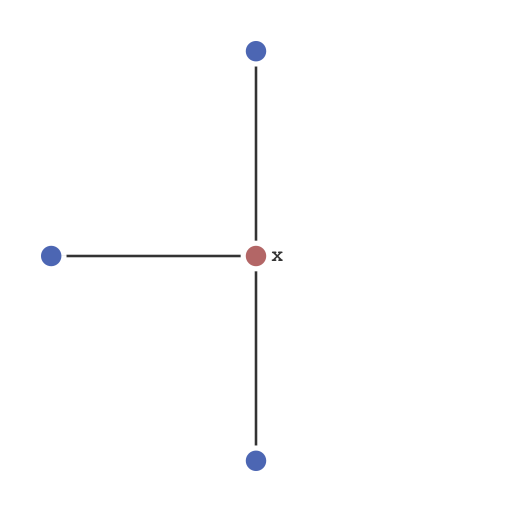
\includegraphics[scale=0.5]{chapters/dyskretna/colours/brooks/images/branching_path.png}
                    \caption{Wierzchołek $x$ ma trzech sąsiadów w kolorze $j$}
                \end{figure}
                
            \item Każde dwa $C_{ij}, C_{ik}, k \neq j$ przecinają się tylko w $v_i$ 
                W przeciwnym razie istnieje wierzchołek $x$ w kolorze $i$,
                który ma dwóch sąsiadów w kolorze $j$ i dwóch sąsiadów w kolorze $k$.
                Jak się dobrze policzy to tak jak poprzednio wyjdzie nam, że jakiś kolor jest wolny i możemy zrobić ten sam myk z przekolorowaniem.
                
                \begin{figure}[ht]
                    \centering
                    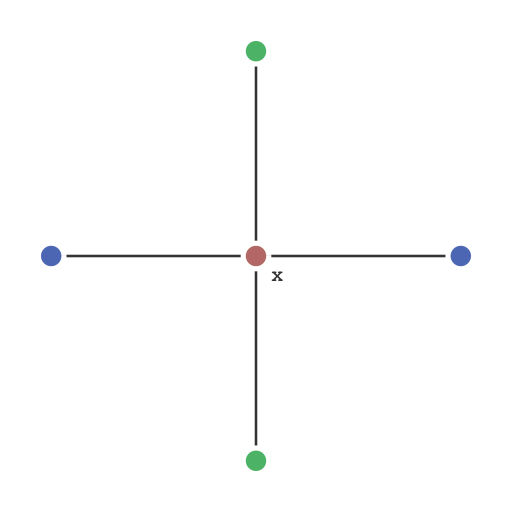
\includegraphics[scale=0.5]{chapters/dyskretna/colours/brooks/images/branching_path_three_colors.png}
                    \caption{Wierzchołek $x$ ma dwóch sąsiadów w kolorze $j$ i dwóch w kolorze $k$}
                \end{figure}
                
            \item Istnieje para $v_i, v_j$, która nie jest połączoną krawędzią. 
                W przeciwnym razie wierzchołki $v, v_1, ..., v_\Delta$ tworzą klikę, co jest sprzeczne z założeniem.
                
                Bez straty ogólności powiedzmy, że $v_1$ i $v_2$ nie są połączone krawędzią. Jednak z własności (5) musi istnieć ścieżka między nimi. Niech więc $u$ to będzie pierwszy wierzchołek w kolorze $1$ na ścieżce od $v_2$ do $v_1$.
                
                Teraz dzieje się magia.
                W $C_{23}$ zamieniamy kolory $2$ i $3$ i takie kolorowanie przepuszczamy przez warunki $(2) - (5)$.
                Jeśli w którymś miejscu udało nam się stworzyć dobre kolorowanie to super, a jeśli nie to ups.
                Na szczęście zauważamy teraz fajną rzecz. Otóż wierzchołek $u$ nadal jest połączony ścieżką w kolorach $1$ i $2$ z wierzchołkiem $v_1$, zatem należy do komponentu $C_{12}$, ale z drugiej strony jest połączony krawędzią z wierzchołkiem $v_2$, który ma teraz kolor $3$ zatem należy też do komponentu $C_{13}$.
                W takim razie nowe kolorowanie narusza warunek $(5)$ co już umiemy rozwiązać.
                
                 \begin{figure}[H]
                    \centering
                    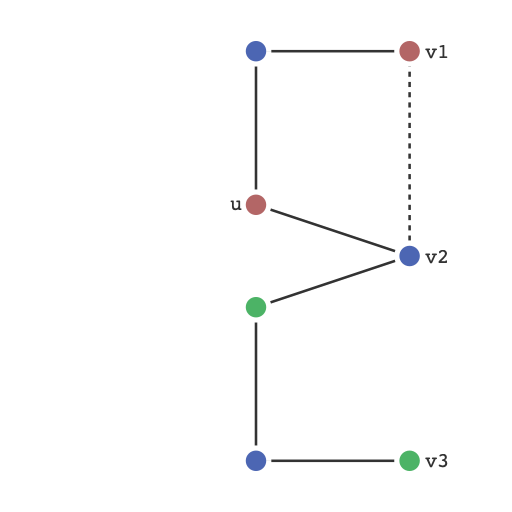
\includegraphics[scale=0.4]{chapters/dyskretna/colours/brooks/images/disconnected_before_swap.png}
                    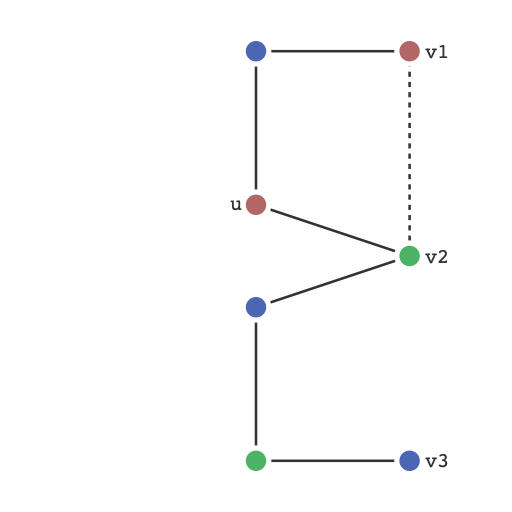
\includegraphics[scale=0.4]{chapters/dyskretna/colours/brooks/images/disconnected_after_swap.png}
                    \caption{Wierzchołki $v_1$ i $v_2$ przed i po przekolorowaniu komponentu $C_{23}$}
                \end{figure}
                
                
        \end{enumerate}
        
        To tyle, nie ma więcej warunków, które musimy rozważać. Fajnie.
        
    \end{proof}

\section{Liczba chromatyczna a liczba kolorująca grafów}
\begin{definition}[Definicja permutacyjna wyznacznika]
Jeśli \(\field\) jest ciałem i \(n \in \natural\), to \textbf{wyznacznikiem} nazwiemy funkcję \(f : \fieldset^{n \times n}\) taką, że:

\[
f(A) = \sum_{\sigma \in S_n} \sgn(\sigma) \cdot A_{1, \; \sigma(1)} \cdot A_{2, \; \sigma(2)} \cdot A_{3, \; \sigma(3)} \cdot \dots \cdot A_{n, \; \sigma(n)} 
\]

gdzie \(A_{ij}\) oznacza komórkę macierzy znajdującą się w \(i\)-tym wierszu i \(j\)-tej kolumnie, a \(S_n\) oznacza zbiór wszystkich permutacji zbioru \(n\)-elementowego.

\end{definition}

\begin{definition}[Definicja ,,objętościowa'' wyznacznika]
Niech \(\field\) będzie ciałem i \(n \in \natural\). Ponadto, niech \(v_1, v_2, v_3, \dots, v_n \in \fieldset^{n}\). Wówczas tuplę \((v_1, v_2, v_3, \dots, v_n) \in (\fieldset^{n})^{n}\) możemy trywialnie utożsamić z macierzą \(M \in \fieldset^{n \times n}\) (i vice versa), poprzez utożsamienie każdego wektora \(\fieldset^{n}\) z pojedynczym wierszem tej macierzy.

Stosując taką notację, mówimy że funkcja \(f: \fieldset^{n \times n} \rightarrow \fieldset\) jest \textbf{wyznacznikiem}, jeśli spełnia następujące warunki: 

\begin{enumerate}
    \item \(f(v_1, v_2, \dots, \lambda v_i, \dots, v_n) = \lambda \cdot f(v_1, v_2, \dots, v_i, \dots, v_n) \)
    \item \(f(v_1, v_2, \dots, v_i + v_{i}', \dots, v_n) = f(v_1, v_2, \dots, v_i, \dots, v_n) + f(v_1, v_2, \dots, v_{i}', \dots, v_n) \)
    \item Jeżeli istnieje takie \(i\), że \(v_i = v_{i+1}\), to \(f(v_1, v_2, \dots, v_i, v_{i+1}, \dots v_n) = 0\)
    \item \(f\) na macierzy identycznościowej przyjmuje wartość \(1\). 
\end{enumerate}

Postulaty te wynikają z chęci stworzenia funkcji obliczającej zorientowaną objętość wielowymiarowego równoległościanu (opisywanego wektorami).

Można wykazać, że dla określonego \(n \in \natural\) istnieje dokładnie 1 funkcja spełniająca wyżej wymienione warunki. Definicja ta okazuje się być równoważna z tą wcześniejszą.

\end{definition}

Wyznacznik oznaczamy jako \(\det\).
\begin{theorem}
Dla dowolnych zbiorów \(A, B, C\) zachodzi
\begin{equation*}
    \pars{A^B}^C \eqnum A^{B \times C}
\end{equation*}
\end{theorem}
\begin{proof}
Z~definicji --- konstruujemy bijekcję
\begin{equation*}
    \alpha\colon \pars{A^B}^C \function A^{B \times C}
\end{equation*}
Funkcja \(\alpha\)~przyjmuje funkcję \(C \function A^B\) i~zwraca funkcję \(B \times C \function A\). Zdefiniujmy \(\alpha\)~następująco:
\begin{equation*}
    \begin{split}
        \alpha\pars{f}
            &\coloneqq \pars{\text{taka funkcja \(\gamma\), że \(\gamma\pars{b, c} = \pars{f\pars{c}}\pars{b}\)}}\\
            &\coloneqq \set{\pars{\pars{b, c}, \pars{f\pars{c}}\pars{b}} : \pars{b, c} \in B \times C}
    \end{split}
\end{equation*}
Nadużywając trochę notacji, możemy to bardziej intuicyjnie zapisać jako
\begin{equation*}
    \pars{\alpha\pars{f}}\pars{b, c} \coloneqq \pars{f\pars{c}}\pars{b}
\end{equation*}
Musimy pokazać, że \(\alpha\)~bijekcją.
\begin{description}
    \item[Injektywność.] Weźmy różne \(f_1, f_2 \in \pars{A^B}^C\) i~pokażmy, że \(\alpha\pars{f_1} \neq \alpha\pars{f_2}\).

        Co to znaczy, że \(f_1, f_2\) są różne? To są funkcje \(C \function A^B\), więc gdy są różne, to na jakimś argumencie \(c_0 \in C\) przyjmują różne wartości:
        \begin{equation*}
            f_1\pars{c_0} \neq f_2\pars{c_0}
        \end{equation*}
        Ale to też są funkcje, tym razem \(B \function A\). Czyli skoro są różne, to na pewnym argumencie \(b_0 \in B\) przyjmują różne wartości:
        \begin{equation*}
            \pars{f_1\pars{c_0}}\pars{b_0} \neq \pars{f_2\pars{c_0}}\pars{b_0}
        \end{equation*}
        Możemy to zapisać za pomocą \(\alpha\)~jako
        \begin{equation*}
            \pars{\alpha\pars{f_1}}\pars{b_0, c_0} \neq \pars{\alpha\pars{f_2}}\pars{b_0, c_0}
        \end{equation*}
        Oznacza to, że funkcje \(\alpha\pars{f_1}, \alpha\pars{f_2}\colon B \times C \function \alpha\) przyjmują różne wartości na argumencie \(\pars{b_0, c_0} \in B \times C\). A~zatem są to różne funkcje \(\alpha\pars{f_1} \neq \alpha\pars{f_2}\), co właśnie chcieliśmy udowodnić.
    \item[Surjektywność.] Weźmy \(g \in A^{B \times C}\). Musimy pokazać, że istnieje \(f \in \pars{A^B}^C\) takie, że
        \begin{equation*}
            \alpha\pars{f} = g
        \end{equation*}
        Niewątpliwie, w~dziedzinie funkcji \(\alpha\)~znajduje się w~szczególności \(f_0\colon C \function A^B\)~zdefiniowane następująco
        \begin{equation*}
            \begin{split}
                f_0\pars{c}
                    &\coloneqq \pars{\text{taka funkcja \(\gamma\), że \(\gamma\pars{b} = g\pars{b, c}\)}}\\
                    &\coloneqq \set{\pars{b, g\pars{b, c}} : b \in B}
            \end{split}
        \end{equation*}
        co można, ponownie z~drobnym nadużyciem notacji można zapisać jako
        \begin{equation*}
            \pars{f_0\pars{c}}\pars{b} \coloneqq g\pars{b, c}
        \end{equation*}
        Zobaczmy, że dla dowolnej pary \(\pars{b_0, c_0} \in B \times C\) zachodzi
        \begin{align*}
            \pars{\alpha\pars{f_0}}\pars{b_0, c_0}
                &= \pars{f_0\pars{c_0}}\pars{b_0} && \text{z~definicji \(\alpha\)}\\
                &= g\pars{b_0, c_0} && \text{z~definicji \(f_0\)}
        \end{align*}
        Zatem istotnie \(\alpha\pars{f_0} = g\) jako funkcje.
\end{description}
\end{proof}
\begin{theorem}
Dla dowolnych zbiorów \(A, B, C\) zachodzi
\begin{equation*}
    \pars{A \times B}^C \eqnum A^C \times B^C
\end{equation*}
\end{theorem}
\begin{proof}
Korzystamy z~przemienności i~konstruujemy bijekcję
\begin{equation*}
    \alpha\colon A^C \times B^C \function \pars{A \times B}^C
\end{equation*}
Funkcja \(\alpha\)~przyjmuje parę funkcji \(\pars{C \function A, C \function B}\) i~zwraca funkcję \(C \function A \times B\). Definiujemy ją następująco:
\begin{equation*}
    \begin{split}
        \alpha\pars{f, g}
            &\coloneqq \pars{\text{taka funkcja \(\eta\), że \(\eta\pars{c} = \pars{f\pars{c}, g\pars{c}}\)}}\\
            &\coloneqq \set{\pars{c, \pars{f\pars{c}, g\pars{c}}} : c \in C}
    \end{split}
\end{equation*}
Inaczej:
\begin{equation*}
    \pars{\alpha\pars{f, g}}\pars{c} = \pars{f\pars{c}, g\pars{c}}
\end{equation*}
Musimy pokazać, że \(\alpha\)~jest bijekcją.
\begin{description}
    \item[Injektywność.] Weźmy różne pary \(\pars{f_1, g_1}, \pars{f_2, g_2} \in A^C \times B^C\). Skoro są to różne pary funkcji, to istnieje takie \(c_0 \in C\), że \(f_1\pars{c_0} \neq f_2\pars{c_0}\) lub istnieje takie \(c_0' \in C\), że \(g_1\pars{c_0'} \neq g_2\pars{c_0'}\). Bez straty ogólności, przyjmijmy pierwszą opcję. Widzimy, że
    \begin{equation*}
        \pars{\alpha\pars{f_1, g_1}}\pars{c_0} = \pars{f_1\pars{c_0}, g_1\pars{c_0}} \neq \pars{f_2\pars{c_0}, g_2\pars{c_0}} = \pars{\alpha\pars{f_2, g_2}}\pars{c_0}
    \end{equation*}
    Oznacza to, że \(\alpha\pars{f_1, g_1}\) i~\(\alpha\pars{f_2, g_2}\) są różnymi funkcjami --- tak, jak chcieliśmy.
    \item[Surjektywność.] Weźmy \(h \in \pars{A \times B}^C\). Musimy pokazać, że istnieje para \(\pars{f_0, g_0} \in A^C \times B^C\) taka, że
        \begin{equation*}
            \alpha\pars{f_0, g_0} = h
        \end{equation*}
        Weźmy
        \begin{gather*}
            f_0\colon C \function A\\
            f_0\pars{c} \coloneqq \text{lewy element pary \(h\pars{c}\)}
        \end{gather*}
        oraz
        \begin{gather*}
            g_0\colon C \function B\\
            g_0\pars{c} \coloneqq \text{prawy element pary \(h\pars{c}\)}
        \end{gather*}
        Teraz dla dowolnego \(c_0 \in C\) mamy
        \begin{equation*}
            \pars{\alpha\pars{f_0, g_0}}\pars{c_0}
                = \pars{f_0\pars{c_0}, g_0\pars{c_0}}
                = \pars{\text{lewy z~\(h\pars{c_0}\)}, \text{prawy z~\(h\pars{c_0}\)}}
                = h\pars{c_0}
        \end{equation*}
        co dowodzi, że \(\alpha\pars{f_0, g_0} = h\) jako funkcje.
        
        Jako bonus możemy zastanowić się, jak teoriomnogościowo wyciągać lewy i~prawy element pary uporządkowanej. Wykorzystamy definicję \ref{mfi:cartesian_and_relations:cartesian_definitions:def:ordered_pair}.
        \begin{itemize}
            \item \(\bigcup\bigcap p\) jest lewym elementem pary \(p\)
                \begin{equation*}
                    p = \pars{a, b} = \set{\set{a}, \set{a, b}} \overset{\bigcap}{\longrightarrow} \set{a} \overset{\bigcup}{\longrightarrow} a
                \end{equation*}
            \item \(\bigcup\pars{\bigcup p \setminus \bigcap p}\) jest prawym elementem pary \(p\)
                \begin{equation*}
                    p = \pars{a, b} = \set{\set{a}, \set{a, b}} \overset{\bigcap}{\longrightarrow} \set{a} \overset{\bigcup \setminus \pars{\mathord{\cdot}}}{\longrightarrow} \set{a, b} \setminus \set{a} = \set{b} \overset{\bigcup}{\longrightarrow} b
                \end{equation*}
        \end{itemize}
\end{description}
\end{proof}



\section{Kolorowania krawędziowe grafów. Twierdzenie Vizinga}
\begin{definition}[Definicja permutacyjna wyznacznika]
Jeśli \(\field\) jest ciałem i \(n \in \natural\), to \textbf{wyznacznikiem} nazwiemy funkcję \(f : \fieldset^{n \times n}\) taką, że:

\[
f(A) = \sum_{\sigma \in S_n} \sgn(\sigma) \cdot A_{1, \; \sigma(1)} \cdot A_{2, \; \sigma(2)} \cdot A_{3, \; \sigma(3)} \cdot \dots \cdot A_{n, \; \sigma(n)} 
\]

gdzie \(A_{ij}\) oznacza komórkę macierzy znajdującą się w \(i\)-tym wierszu i \(j\)-tej kolumnie, a \(S_n\) oznacza zbiór wszystkich permutacji zbioru \(n\)-elementowego.

\end{definition}

\begin{definition}[Definicja ,,objętościowa'' wyznacznika]
Niech \(\field\) będzie ciałem i \(n \in \natural\). Ponadto, niech \(v_1, v_2, v_3, \dots, v_n \in \fieldset^{n}\). Wówczas tuplę \((v_1, v_2, v_3, \dots, v_n) \in (\fieldset^{n})^{n}\) możemy trywialnie utożsamić z macierzą \(M \in \fieldset^{n \times n}\) (i vice versa), poprzez utożsamienie każdego wektora \(\fieldset^{n}\) z pojedynczym wierszem tej macierzy.

Stosując taką notację, mówimy że funkcja \(f: \fieldset^{n \times n} \rightarrow \fieldset\) jest \textbf{wyznacznikiem}, jeśli spełnia następujące warunki: 

\begin{enumerate}
    \item \(f(v_1, v_2, \dots, \lambda v_i, \dots, v_n) = \lambda \cdot f(v_1, v_2, \dots, v_i, \dots, v_n) \)
    \item \(f(v_1, v_2, \dots, v_i + v_{i}', \dots, v_n) = f(v_1, v_2, \dots, v_i, \dots, v_n) + f(v_1, v_2, \dots, v_{i}', \dots, v_n) \)
    \item Jeżeli istnieje takie \(i\), że \(v_i = v_{i+1}\), to \(f(v_1, v_2, \dots, v_i, v_{i+1}, \dots v_n) = 0\)
    \item \(f\) na macierzy identycznościowej przyjmuje wartość \(1\). 
\end{enumerate}

Postulaty te wynikają z chęci stworzenia funkcji obliczającej zorientowaną objętość wielowymiarowego równoległościanu (opisywanego wektorami).

Można wykazać, że dla określonego \(n \in \natural\) istnieje dokładnie 1 funkcja spełniająca wyżej wymienione warunki. Definicja ta okazuje się być równoważna z tą wcześniejszą.

\end{definition}

Wyznacznik oznaczamy jako \(\det\).
\begin{theorem}
Dla dowolnych zbiorów \(A, B, C\) zachodzi
\begin{equation*}
    \pars{A^B}^C \eqnum A^{B \times C}
\end{equation*}
\end{theorem}
\begin{proof}
Z~definicji --- konstruujemy bijekcję
\begin{equation*}
    \alpha\colon \pars{A^B}^C \function A^{B \times C}
\end{equation*}
Funkcja \(\alpha\)~przyjmuje funkcję \(C \function A^B\) i~zwraca funkcję \(B \times C \function A\). Zdefiniujmy \(\alpha\)~następująco:
\begin{equation*}
    \begin{split}
        \alpha\pars{f}
            &\coloneqq \pars{\text{taka funkcja \(\gamma\), że \(\gamma\pars{b, c} = \pars{f\pars{c}}\pars{b}\)}}\\
            &\coloneqq \set{\pars{\pars{b, c}, \pars{f\pars{c}}\pars{b}} : \pars{b, c} \in B \times C}
    \end{split}
\end{equation*}
Nadużywając trochę notacji, możemy to bardziej intuicyjnie zapisać jako
\begin{equation*}
    \pars{\alpha\pars{f}}\pars{b, c} \coloneqq \pars{f\pars{c}}\pars{b}
\end{equation*}
Musimy pokazać, że \(\alpha\)~bijekcją.
\begin{description}
    \item[Injektywność.] Weźmy różne \(f_1, f_2 \in \pars{A^B}^C\) i~pokażmy, że \(\alpha\pars{f_1} \neq \alpha\pars{f_2}\).

        Co to znaczy, że \(f_1, f_2\) są różne? To są funkcje \(C \function A^B\), więc gdy są różne, to na jakimś argumencie \(c_0 \in C\) przyjmują różne wartości:
        \begin{equation*}
            f_1\pars{c_0} \neq f_2\pars{c_0}
        \end{equation*}
        Ale to też są funkcje, tym razem \(B \function A\). Czyli skoro są różne, to na pewnym argumencie \(b_0 \in B\) przyjmują różne wartości:
        \begin{equation*}
            \pars{f_1\pars{c_0}}\pars{b_0} \neq \pars{f_2\pars{c_0}}\pars{b_0}
        \end{equation*}
        Możemy to zapisać za pomocą \(\alpha\)~jako
        \begin{equation*}
            \pars{\alpha\pars{f_1}}\pars{b_0, c_0} \neq \pars{\alpha\pars{f_2}}\pars{b_0, c_0}
        \end{equation*}
        Oznacza to, że funkcje \(\alpha\pars{f_1}, \alpha\pars{f_2}\colon B \times C \function \alpha\) przyjmują różne wartości na argumencie \(\pars{b_0, c_0} \in B \times C\). A~zatem są to różne funkcje \(\alpha\pars{f_1} \neq \alpha\pars{f_2}\), co właśnie chcieliśmy udowodnić.
    \item[Surjektywność.] Weźmy \(g \in A^{B \times C}\). Musimy pokazać, że istnieje \(f \in \pars{A^B}^C\) takie, że
        \begin{equation*}
            \alpha\pars{f} = g
        \end{equation*}
        Niewątpliwie, w~dziedzinie funkcji \(\alpha\)~znajduje się w~szczególności \(f_0\colon C \function A^B\)~zdefiniowane następująco
        \begin{equation*}
            \begin{split}
                f_0\pars{c}
                    &\coloneqq \pars{\text{taka funkcja \(\gamma\), że \(\gamma\pars{b} = g\pars{b, c}\)}}\\
                    &\coloneqq \set{\pars{b, g\pars{b, c}} : b \in B}
            \end{split}
        \end{equation*}
        co można, ponownie z~drobnym nadużyciem notacji można zapisać jako
        \begin{equation*}
            \pars{f_0\pars{c}}\pars{b} \coloneqq g\pars{b, c}
        \end{equation*}
        Zobaczmy, że dla dowolnej pary \(\pars{b_0, c_0} \in B \times C\) zachodzi
        \begin{align*}
            \pars{\alpha\pars{f_0}}\pars{b_0, c_0}
                &= \pars{f_0\pars{c_0}}\pars{b_0} && \text{z~definicji \(\alpha\)}\\
                &= g\pars{b_0, c_0} && \text{z~definicji \(f_0\)}
        \end{align*}
        Zatem istotnie \(\alpha\pars{f_0} = g\) jako funkcje.
\end{description}
\end{proof}
\begin{theorem}
Dla dowolnych zbiorów \(A, B, C\) zachodzi
\begin{equation*}
    \pars{A \times B}^C \eqnum A^C \times B^C
\end{equation*}
\end{theorem}
\begin{proof}
Korzystamy z~przemienności i~konstruujemy bijekcję
\begin{equation*}
    \alpha\colon A^C \times B^C \function \pars{A \times B}^C
\end{equation*}
Funkcja \(\alpha\)~przyjmuje parę funkcji \(\pars{C \function A, C \function B}\) i~zwraca funkcję \(C \function A \times B\). Definiujemy ją następująco:
\begin{equation*}
    \begin{split}
        \alpha\pars{f, g}
            &\coloneqq \pars{\text{taka funkcja \(\eta\), że \(\eta\pars{c} = \pars{f\pars{c}, g\pars{c}}\)}}\\
            &\coloneqq \set{\pars{c, \pars{f\pars{c}, g\pars{c}}} : c \in C}
    \end{split}
\end{equation*}
Inaczej:
\begin{equation*}
    \pars{\alpha\pars{f, g}}\pars{c} = \pars{f\pars{c}, g\pars{c}}
\end{equation*}
Musimy pokazać, że \(\alpha\)~jest bijekcją.
\begin{description}
    \item[Injektywność.] Weźmy różne pary \(\pars{f_1, g_1}, \pars{f_2, g_2} \in A^C \times B^C\). Skoro są to różne pary funkcji, to istnieje takie \(c_0 \in C\), że \(f_1\pars{c_0} \neq f_2\pars{c_0}\) lub istnieje takie \(c_0' \in C\), że \(g_1\pars{c_0'} \neq g_2\pars{c_0'}\). Bez straty ogólności, przyjmijmy pierwszą opcję. Widzimy, że
    \begin{equation*}
        \pars{\alpha\pars{f_1, g_1}}\pars{c_0} = \pars{f_1\pars{c_0}, g_1\pars{c_0}} \neq \pars{f_2\pars{c_0}, g_2\pars{c_0}} = \pars{\alpha\pars{f_2, g_2}}\pars{c_0}
    \end{equation*}
    Oznacza to, że \(\alpha\pars{f_1, g_1}\) i~\(\alpha\pars{f_2, g_2}\) są różnymi funkcjami --- tak, jak chcieliśmy.
    \item[Surjektywność.] Weźmy \(h \in \pars{A \times B}^C\). Musimy pokazać, że istnieje para \(\pars{f_0, g_0} \in A^C \times B^C\) taka, że
        \begin{equation*}
            \alpha\pars{f_0, g_0} = h
        \end{equation*}
        Weźmy
        \begin{gather*}
            f_0\colon C \function A\\
            f_0\pars{c} \coloneqq \text{lewy element pary \(h\pars{c}\)}
        \end{gather*}
        oraz
        \begin{gather*}
            g_0\colon C \function B\\
            g_0\pars{c} \coloneqq \text{prawy element pary \(h\pars{c}\)}
        \end{gather*}
        Teraz dla dowolnego \(c_0 \in C\) mamy
        \begin{equation*}
            \pars{\alpha\pars{f_0, g_0}}\pars{c_0}
                = \pars{f_0\pars{c_0}, g_0\pars{c_0}}
                = \pars{\text{lewy z~\(h\pars{c_0}\)}, \text{prawy z~\(h\pars{c_0}\)}}
                = h\pars{c_0}
        \end{equation*}
        co dowodzi, że \(\alpha\pars{f_0, g_0} = h\) jako funkcje.
        
        Jako bonus możemy zastanowić się, jak teoriomnogościowo wyciągać lewy i~prawy element pary uporządkowanej. Wykorzystamy definicję \ref{mfi:cartesian_and_relations:cartesian_definitions:def:ordered_pair}.
        \begin{itemize}
            \item \(\bigcup\bigcap p\) jest lewym elementem pary \(p\)
                \begin{equation*}
                    p = \pars{a, b} = \set{\set{a}, \set{a, b}} \overset{\bigcap}{\longrightarrow} \set{a} \overset{\bigcup}{\longrightarrow} a
                \end{equation*}
            \item \(\bigcup\pars{\bigcup p \setminus \bigcap p}\) jest prawym elementem pary \(p\)
                \begin{equation*}
                    p = \pars{a, b} = \set{\set{a}, \set{a, b}} \overset{\bigcap}{\longrightarrow} \set{a} \overset{\bigcup \setminus \pars{\mathord{\cdot}}}{\longrightarrow} \set{a, b} \setminus \set{a} = \set{b} \overset{\bigcup}{\longrightarrow} b
                \end{equation*}
        \end{itemize}
\end{description}
\end{proof}



\section{Przepływy w sieciach. Twierdzenie o maksymalnym przepływie i minimalnym
przekroju}
\begin{definition}[Definicja permutacyjna wyznacznika]
Jeśli \(\field\) jest ciałem i \(n \in \natural\), to \textbf{wyznacznikiem} nazwiemy funkcję \(f : \fieldset^{n \times n}\) taką, że:

\[
f(A) = \sum_{\sigma \in S_n} \sgn(\sigma) \cdot A_{1, \; \sigma(1)} \cdot A_{2, \; \sigma(2)} \cdot A_{3, \; \sigma(3)} \cdot \dots \cdot A_{n, \; \sigma(n)} 
\]

gdzie \(A_{ij}\) oznacza komórkę macierzy znajdującą się w \(i\)-tym wierszu i \(j\)-tej kolumnie, a \(S_n\) oznacza zbiór wszystkich permutacji zbioru \(n\)-elementowego.

\end{definition}

\begin{definition}[Definicja ,,objętościowa'' wyznacznika]
Niech \(\field\) będzie ciałem i \(n \in \natural\). Ponadto, niech \(v_1, v_2, v_3, \dots, v_n \in \fieldset^{n}\). Wówczas tuplę \((v_1, v_2, v_3, \dots, v_n) \in (\fieldset^{n})^{n}\) możemy trywialnie utożsamić z macierzą \(M \in \fieldset^{n \times n}\) (i vice versa), poprzez utożsamienie każdego wektora \(\fieldset^{n}\) z pojedynczym wierszem tej macierzy.

Stosując taką notację, mówimy że funkcja \(f: \fieldset^{n \times n} \rightarrow \fieldset\) jest \textbf{wyznacznikiem}, jeśli spełnia następujące warunki: 

\begin{enumerate}
    \item \(f(v_1, v_2, \dots, \lambda v_i, \dots, v_n) = \lambda \cdot f(v_1, v_2, \dots, v_i, \dots, v_n) \)
    \item \(f(v_1, v_2, \dots, v_i + v_{i}', \dots, v_n) = f(v_1, v_2, \dots, v_i, \dots, v_n) + f(v_1, v_2, \dots, v_{i}', \dots, v_n) \)
    \item Jeżeli istnieje takie \(i\), że \(v_i = v_{i+1}\), to \(f(v_1, v_2, \dots, v_i, v_{i+1}, \dots v_n) = 0\)
    \item \(f\) na macierzy identycznościowej przyjmuje wartość \(1\). 
\end{enumerate}

Postulaty te wynikają z chęci stworzenia funkcji obliczającej zorientowaną objętość wielowymiarowego równoległościanu (opisywanego wektorami).

Można wykazać, że dla określonego \(n \in \natural\) istnieje dokładnie 1 funkcja spełniająca wyżej wymienione warunki. Definicja ta okazuje się być równoważna z tą wcześniejszą.

\end{definition}

Wyznacznik oznaczamy jako \(\det\).
\begin{theorem}
Dla dowolnych zbiorów \(A, B, C\) zachodzi
\begin{equation*}
    \pars{A^B}^C \eqnum A^{B \times C}
\end{equation*}
\end{theorem}
\begin{proof}
Z~definicji --- konstruujemy bijekcję
\begin{equation*}
    \alpha\colon \pars{A^B}^C \function A^{B \times C}
\end{equation*}
Funkcja \(\alpha\)~przyjmuje funkcję \(C \function A^B\) i~zwraca funkcję \(B \times C \function A\). Zdefiniujmy \(\alpha\)~następująco:
\begin{equation*}
    \begin{split}
        \alpha\pars{f}
            &\coloneqq \pars{\text{taka funkcja \(\gamma\), że \(\gamma\pars{b, c} = \pars{f\pars{c}}\pars{b}\)}}\\
            &\coloneqq \set{\pars{\pars{b, c}, \pars{f\pars{c}}\pars{b}} : \pars{b, c} \in B \times C}
    \end{split}
\end{equation*}
Nadużywając trochę notacji, możemy to bardziej intuicyjnie zapisać jako
\begin{equation*}
    \pars{\alpha\pars{f}}\pars{b, c} \coloneqq \pars{f\pars{c}}\pars{b}
\end{equation*}
Musimy pokazać, że \(\alpha\)~bijekcją.
\begin{description}
    \item[Injektywność.] Weźmy różne \(f_1, f_2 \in \pars{A^B}^C\) i~pokażmy, że \(\alpha\pars{f_1} \neq \alpha\pars{f_2}\).

        Co to znaczy, że \(f_1, f_2\) są różne? To są funkcje \(C \function A^B\), więc gdy są różne, to na jakimś argumencie \(c_0 \in C\) przyjmują różne wartości:
        \begin{equation*}
            f_1\pars{c_0} \neq f_2\pars{c_0}
        \end{equation*}
        Ale to też są funkcje, tym razem \(B \function A\). Czyli skoro są różne, to na pewnym argumencie \(b_0 \in B\) przyjmują różne wartości:
        \begin{equation*}
            \pars{f_1\pars{c_0}}\pars{b_0} \neq \pars{f_2\pars{c_0}}\pars{b_0}
        \end{equation*}
        Możemy to zapisać za pomocą \(\alpha\)~jako
        \begin{equation*}
            \pars{\alpha\pars{f_1}}\pars{b_0, c_0} \neq \pars{\alpha\pars{f_2}}\pars{b_0, c_0}
        \end{equation*}
        Oznacza to, że funkcje \(\alpha\pars{f_1}, \alpha\pars{f_2}\colon B \times C \function \alpha\) przyjmują różne wartości na argumencie \(\pars{b_0, c_0} \in B \times C\). A~zatem są to różne funkcje \(\alpha\pars{f_1} \neq \alpha\pars{f_2}\), co właśnie chcieliśmy udowodnić.
    \item[Surjektywność.] Weźmy \(g \in A^{B \times C}\). Musimy pokazać, że istnieje \(f \in \pars{A^B}^C\) takie, że
        \begin{equation*}
            \alpha\pars{f} = g
        \end{equation*}
        Niewątpliwie, w~dziedzinie funkcji \(\alpha\)~znajduje się w~szczególności \(f_0\colon C \function A^B\)~zdefiniowane następująco
        \begin{equation*}
            \begin{split}
                f_0\pars{c}
                    &\coloneqq \pars{\text{taka funkcja \(\gamma\), że \(\gamma\pars{b} = g\pars{b, c}\)}}\\
                    &\coloneqq \set{\pars{b, g\pars{b, c}} : b \in B}
            \end{split}
        \end{equation*}
        co można, ponownie z~drobnym nadużyciem notacji można zapisać jako
        \begin{equation*}
            \pars{f_0\pars{c}}\pars{b} \coloneqq g\pars{b, c}
        \end{equation*}
        Zobaczmy, że dla dowolnej pary \(\pars{b_0, c_0} \in B \times C\) zachodzi
        \begin{align*}
            \pars{\alpha\pars{f_0}}\pars{b_0, c_0}
                &= \pars{f_0\pars{c_0}}\pars{b_0} && \text{z~definicji \(\alpha\)}\\
                &= g\pars{b_0, c_0} && \text{z~definicji \(f_0\)}
        \end{align*}
        Zatem istotnie \(\alpha\pars{f_0} = g\) jako funkcje.
\end{description}
\end{proof}
\begin{theorem}
Dla dowolnych zbiorów \(A, B, C\) zachodzi
\begin{equation*}
    \pars{A \times B}^C \eqnum A^C \times B^C
\end{equation*}
\end{theorem}
\begin{proof}
Korzystamy z~przemienności i~konstruujemy bijekcję
\begin{equation*}
    \alpha\colon A^C \times B^C \function \pars{A \times B}^C
\end{equation*}
Funkcja \(\alpha\)~przyjmuje parę funkcji \(\pars{C \function A, C \function B}\) i~zwraca funkcję \(C \function A \times B\). Definiujemy ją następująco:
\begin{equation*}
    \begin{split}
        \alpha\pars{f, g}
            &\coloneqq \pars{\text{taka funkcja \(\eta\), że \(\eta\pars{c} = \pars{f\pars{c}, g\pars{c}}\)}}\\
            &\coloneqq \set{\pars{c, \pars{f\pars{c}, g\pars{c}}} : c \in C}
    \end{split}
\end{equation*}
Inaczej:
\begin{equation*}
    \pars{\alpha\pars{f, g}}\pars{c} = \pars{f\pars{c}, g\pars{c}}
\end{equation*}
Musimy pokazać, że \(\alpha\)~jest bijekcją.
\begin{description}
    \item[Injektywność.] Weźmy różne pary \(\pars{f_1, g_1}, \pars{f_2, g_2} \in A^C \times B^C\). Skoro są to różne pary funkcji, to istnieje takie \(c_0 \in C\), że \(f_1\pars{c_0} \neq f_2\pars{c_0}\) lub istnieje takie \(c_0' \in C\), że \(g_1\pars{c_0'} \neq g_2\pars{c_0'}\). Bez straty ogólności, przyjmijmy pierwszą opcję. Widzimy, że
    \begin{equation*}
        \pars{\alpha\pars{f_1, g_1}}\pars{c_0} = \pars{f_1\pars{c_0}, g_1\pars{c_0}} \neq \pars{f_2\pars{c_0}, g_2\pars{c_0}} = \pars{\alpha\pars{f_2, g_2}}\pars{c_0}
    \end{equation*}
    Oznacza to, że \(\alpha\pars{f_1, g_1}\) i~\(\alpha\pars{f_2, g_2}\) są różnymi funkcjami --- tak, jak chcieliśmy.
    \item[Surjektywność.] Weźmy \(h \in \pars{A \times B}^C\). Musimy pokazać, że istnieje para \(\pars{f_0, g_0} \in A^C \times B^C\) taka, że
        \begin{equation*}
            \alpha\pars{f_0, g_0} = h
        \end{equation*}
        Weźmy
        \begin{gather*}
            f_0\colon C \function A\\
            f_0\pars{c} \coloneqq \text{lewy element pary \(h\pars{c}\)}
        \end{gather*}
        oraz
        \begin{gather*}
            g_0\colon C \function B\\
            g_0\pars{c} \coloneqq \text{prawy element pary \(h\pars{c}\)}
        \end{gather*}
        Teraz dla dowolnego \(c_0 \in C\) mamy
        \begin{equation*}
            \pars{\alpha\pars{f_0, g_0}}\pars{c_0}
                = \pars{f_0\pars{c_0}, g_0\pars{c_0}}
                = \pars{\text{lewy z~\(h\pars{c_0}\)}, \text{prawy z~\(h\pars{c_0}\)}}
                = h\pars{c_0}
        \end{equation*}
        co dowodzi, że \(\alpha\pars{f_0, g_0} = h\) jako funkcje.
        
        Jako bonus możemy zastanowić się, jak teoriomnogościowo wyciągać lewy i~prawy element pary uporządkowanej. Wykorzystamy definicję \ref{mfi:cartesian_and_relations:cartesian_definitions:def:ordered_pair}.
        \begin{itemize}
            \item \(\bigcup\bigcap p\) jest lewym elementem pary \(p\)
                \begin{equation*}
                    p = \pars{a, b} = \set{\set{a}, \set{a, b}} \overset{\bigcap}{\longrightarrow} \set{a} \overset{\bigcup}{\longrightarrow} a
                \end{equation*}
            \item \(\bigcup\pars{\bigcup p \setminus \bigcap p}\) jest prawym elementem pary \(p\)
                \begin{equation*}
                    p = \pars{a, b} = \set{\set{a}, \set{a, b}} \overset{\bigcap}{\longrightarrow} \set{a} \overset{\bigcup \setminus \pars{\mathord{\cdot}}}{\longrightarrow} \set{a, b} \setminus \set{a} = \set{b} \overset{\bigcup}{\longrightarrow} b
                \end{equation*}
        \end{itemize}
\end{description}
\end{proof}

